\documentclass[12pt,a4paper]{article}

\usepackage[italian]{babel}
\usepackage[T1]{fontenc}
\usepackage[utf8]{inputenc}
\usepackage{lmodern}
\usepackage{geometry}
\usepackage{setspace}
\usepackage{graphicx}
\usepackage{float}
\usepackage{hyperref}
\usepackage{booktabs}
\usepackage[table]{xcolor}
\usepackage{listings}
\usepackage{caption}
\usepackage{subcaption}
\usepackage{enumitem}
\usepackage{longtable}
\usepackage{array}
\usepackage{microtype}
\usepackage{fancyhdr}
\usepackage{amsmath}
\usepackage{tabularx}


% PER CAMBIARE LA GRANDEZZA DEL TESTO NEGLI SNIPPET DI CODICE
\newcommand{\codesize}{\footnotesize} 


% ---- IntelliJ Light ----
\definecolor{ijLtKeyword}{HTML}{000080}
\definecolor{ijLtString}{HTML}{067D17}
\definecolor{ijLtComment}{HTML}{8C8C8C}
\definecolor{ijLtNumber}{HTML}{1750EB}
\definecolor{ijLtAnnot}{HTML}{9E880D}
\definecolor{ijLtText}{HTML}{080808}
\definecolor{ijLtBg}{HTML}{FFFFFF}
\definecolor{ijLtLineNo}{HTML}{999999}
\definecolor{ijLtFrame}{HTML}{C9C9C9}

% ---- IntelliJ Darcula ----
\definecolor{ijDkKeyword}{HTML}{CC7832}
\definecolor{ijDkString}{HTML}{6A8759}
\definecolor{ijDkComment}{HTML}{808080}
\definecolor{ijDkNumber}{HTML}{6897BB}
\definecolor{ijDkAnnot}{HTML}{BBB529}
\definecolor{ijDkText}{HTML}{A9B7C6}
\definecolor{ijDkBg}{HTML}{2B2B2B}
\definecolor{ijDkLineNo}{HTML}{606366}
\definecolor{ijDkFrame}{HTML}{555555}

% ---- Shared layout (numbers inside the box) ----
\lstdefinestyle{javabase}{
  language=Java,
  alsoletter={@},
  morekeywords=[2]{@Override,@Deprecated,@FunctionalInterface,@SuppressWarnings,@SafeVarargs},
  numbers=left, stepnumber=1, numbersep=6pt,
  xleftmargin=22pt, framexleftmargin=22pt,
  frame=single, framesep=6pt,
  basicstyle=\ttfamily\codesize,
  breaklines=true, tabsize=4, showstringspaces=false,
  captionpos=b
}

\lstdefinestyle{intellijlight}{
  style=javabase,
  backgroundcolor=\color{ijLtBg},
  rulecolor=\color{ijLtFrame},
  basicstyle=\ttfamily\codesize\color{ijLtText},
  keywordstyle=\color{ijLtKeyword}\bfseries,
  keywordstyle=[2]\color{ijLtAnnot},
  stringstyle=\color{ijLtString},
  commentstyle=\color{ijLtComment}\itshape,
  numberstyle=\tiny\color{ijLtLineNo}
}

\lstdefinestyle{intellijdark}{
  style=javabase,
  backgroundcolor=\color{ijDkBg},
  rulecolor=\color{ijDkFrame},
  basicstyle=\ttfamily\codesize\color{ijDkText},
  keywordstyle=\color{ijDkKeyword},          % Darcula keywords are not bold
  keywordstyle=[2]\color{ijDkAnnot},
  stringstyle=\color{ijDkString},
  commentstyle=\color{ijDkComment}\itshape,
  numberstyle=\tiny\color{ijDkLineNo}
}



\geometry{margin=2.4cm}
\onehalfspacing
\setlength{\emergencystretch}{3em}
\graphicspath{{img/}}
\hypersetup{
  colorlinks=true,
  linkcolor=black,
  urlcolor=blue!65!black,
  citecolor=blue!55!black,
  pdftitle={MBPConfigurator - Relazione di Ingegneria del Software},
  pdfauthor={Tommaso Lapenna, Lucas Melo Alves, Samuele Baldi}
}

\pagestyle{fancy}
\fancyhf{}
\fancyhead[L]{MPBConfigurator}
\fancyhead[R]{Ingegneria del Software}
\fancyfoot[C]{\thepage}
\setlength{\headheight}{15pt}

\definecolor{codebg}{RGB}{247,248,250}
\definecolor{codeframe}{RGB}{190,198,205}
\lstdefinestyle{codeStyle}{
  basicstyle=\ttfamily\footnotesize,
  backgroundcolor=\color{codebg},
  breaklines=true,
  frame=single,
  rulecolor=\color{codeframe},
  tabsize=2,
  numbers=left,
  numberstyle=\tiny\color{gray},
  keywordstyle=\color{blue!70!black},
  commentstyle=\color{green!40!black},
  stringstyle=\color{orange!70!black},
  showstringspaces=false,
  columns=fullflexible
}

\newcommand{\project}{\textbf{MBPConfigurator}}
\newcommand{\code}[1]{\nolinkurl{#1}}
\newcommand{\HRule}{\rule{\linewidth}{0.5mm}}

\title{
  \vspace{1.5cm}
  {\Huge\textbf{MBPConfigurator}}\\[0.4cm]
  {\Large}\\[1.5cm]
  {\large Relazione di Ingegneria del Software}
}
\author{
  Tommaso Lapenna\\
  Corso di Laurea in Ingegneria Informatica\\
  Università degli Studi di Firenze
}
\date{Anno Accademico 2025--2026}

\begin{document}

\begin{titlepage}
\newgeometry{top=2.5cm,bottom=2.5cm,left=3cm,right=3cm}
\thispagestyle{empty}
\begin{center}

\IfFileExists{logounifi.png}{
  
\includegraphics[width=0.48\textwidth]{logounifi.png}\\[0.6cm]
}{
  \vspace*{1.2cm}
}

\textsc{\LARGE Università degli Studi di Firenze}\\[0.45cm]
\textsc{\Large Dipartimento di Ingegneria dell'Informazione}\\[1.2cm]

\HRule\\[0.8cm]
{\Huge\bfseries MBPConfigurator}\\[0.35cm]
{\Large Configuratore di PC}\\[0.8cm]
\HRule\\[1.6cm]

\begin{minipage}[t]{0.46\textwidth}
  \begin{flushleft}\large
    \emph{Autori:}\\
    Tommaso Lapenna\\
    Lucas Melo Alves\\
    Samuele Baldi\\[1.2em]
    \emph{N\textsuperscript{o} matricola:}\\
    7112937\\
    7777777\\
    7116707
  \end{flushleft}
\end{minipage}
\hfill
\begin{minipage}[t]{0.46\textwidth}
  \begin{flushright}\large
    \emph{Corso:}\\
    Ingegneria del Software\\[1.2em]
    \emph{Docente del corso:}\\
    Prof.\ Enrico Vicario
  \end{flushright}
\end{minipage}

\vfill
{\large Anno Accademico 2025--2026}

\end{center}
\restoregeometry
\end{titlepage}

\newpage

\tableofcontents
\newpage
\section{Introduzione}
\subsection{Statement}
Il progetto \textbf{MPBConfigurator} modella un'applicazione che permette all'utente di creare una pc build, confrontare i componenti e verificarne la compatibilità ed il prezzo totale.

L'interfaccia del configuratore permette di inserire via via i componenti scelti, annullare le scelte effettuate o ripristinare l'annullamento. Inoltre sono visibili informazioni su cosa modificare e/o inserire per ottenere un pc funzionante tramite il sistema di compatibilità in tempo reale.

Tutto il catalogo dei componenti è disponibile all'utente tramite l'apposito database, quest'ultimo è gestito dall'operatore del sistema.

\subsection{Obiettivo e Requisiti}
???? maybe?

\subsection{Tecnologie e Strumenti Utilizzati}

\begin{table}[H]
    \centering
    \begin{tabular}{|c|c|}
    \hline
        Java 25 &  Implementazione dell'applicazione \\
        \hline
        IntelliJ & IDE \\
        \hline
        JUnit 5 &  Testing dell'applicazione \\
        \hline
        SQLite  &  Database dell'applicazione\\
        \hline
        PlantUML & Strumento di creazione dei diagrammi UML \\
        \hline
        Github & Versionamento e condivisione del codice\\
        \hline
    \end{tabular}
    \caption{Tecnologie utilizzate}
    \label{tab:placeholder}
\end{table}



Sono inoltre stati utilizzati i seguenti modelli per aiutare lo sviluppo del codice e la progettazione:
\begin{itemize}
    \item Claude Sonnet 5.5
    \item Claude Agent
    \item Gemini Pro 3.1, Flash 3.5
    \item LLM locali: (Gemma 4 e4b, Qwen 3.5 9b, Nemotron 3-nano 4b)
\end{itemize}



\begin{itemize}
    \item \textbf{GUI} rappresenta l'UI layer.
    \item \textbf{Application} rappresenta l'Application Layer, e si occuppa di gestire le richieste dell'utente e la coordinazioni tra i vari elementi (in modo da "risolvere" gli use cases).
    \item \textbf{Domain} rappresenta il Domain Layer: contiene il modello di tutte le entità del dominio in questione (tutti i tipi di componenti e le build), insieme a tutta la logica e regole che le gestiscono.
    \item \textbf{ORM} rappresenta il Persisistence Layer, definisce le repository interfaces deinite dal dominio.
\end{itemize}



\section{Progettazione}
\subsection{Architettura e Design}

L'applicazione è strutturata secondo un'architettura a livelli, inspirata al Domain Driven Desgin

\begin{figure}[H]
    \centering
    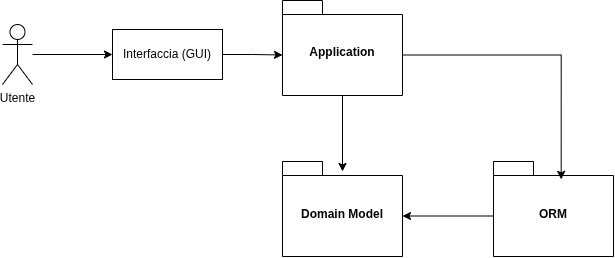
\includegraphics[width=1\linewidth]{diagrammi/packagediagram-light.png}
    \caption{Package Diagram}
    \label{fig:placeholder}
\end{figure}
NEL DIAGRAMMA MANCA IL DB

DEFINIZIONE LAYER
\subsection{Use Case Diagram}
\begin{figure}[H]
    \centering
    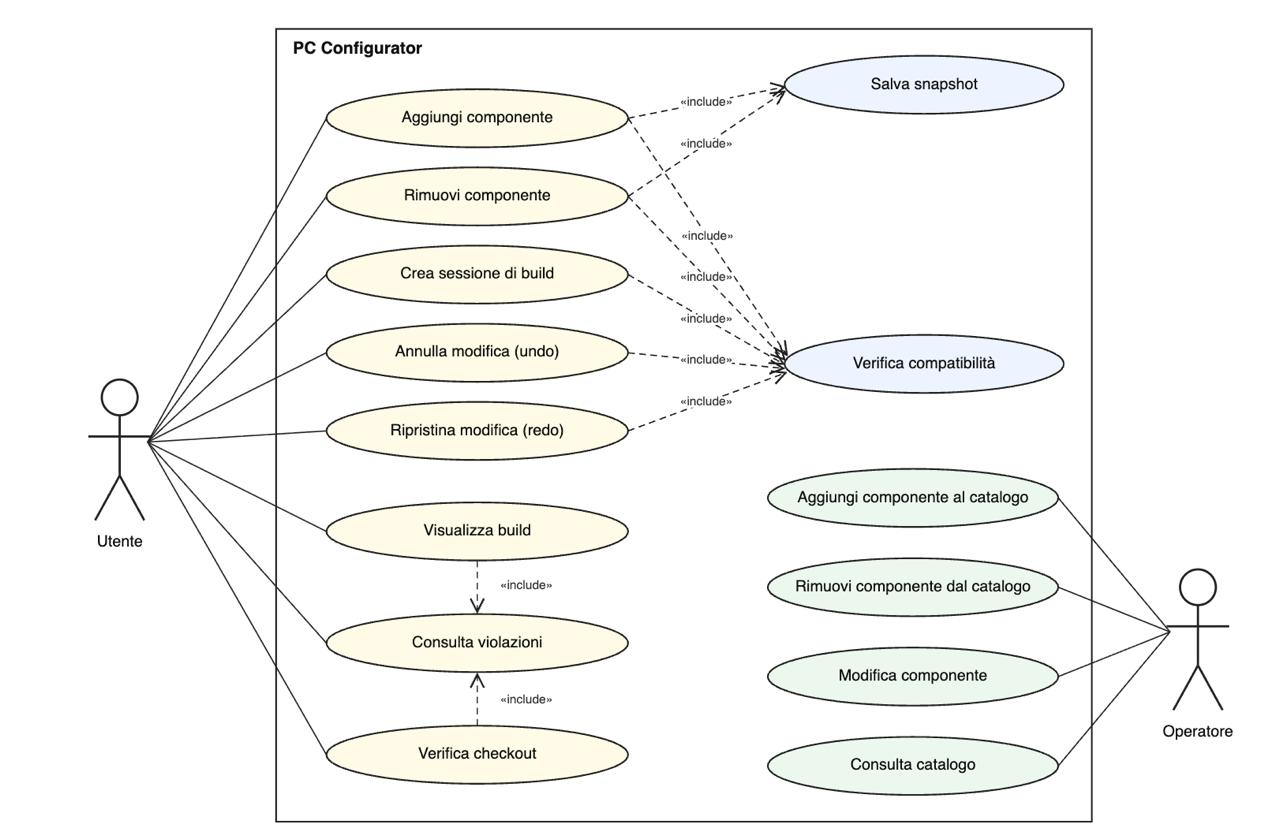
\includegraphics[width=0.75\linewidth]{diagrammi/usecases.png}
    \caption{Use Case Diagram}
    \label{fig:placeholder}
\end{figure}

\subsection{Use Case Template}
{
\singlespacing
\footnotesize
\renewcommand{\arraystretch}{1.1}
\vspace{8pt}
% UC1
\noindent
\begin{tabularx}{\textwidth}{|>{\bfseries}p{3.8cm}|X|}
\hline
\multicolumn{2}{|l|}{\textbf{UC1 --- Crea sessione di build}} \\
\hline
Descrizione & L'utente avvia una nuova sessione di configurazione PC. Il sistema crea una \texttt{PcBuildSession} vuota con \texttt{PcBuilder} e \texttt{SnapshotHistory} inizializzati. \\
\hline
Livello & User goal \\
\hline
Attori & Utente \\
\hline
Pre-condizioni & L'utente è autenticato nel sistema. \\
\hline
Flusso base & 1. L'utente seleziona «Nuova build».\newline 2. Il sistema crea una \texttt{PcBuildSession} con \texttt{PcBuilder} vuoto.\newline 3. Il sistema inizializza la \texttt{SnapshotHistory}.\newline 4. Il sistema mostra l'interfaccia di configurazione con tutti gli slot vuoti. \\
\hline
Flussi alternativi & 1a. L'utente sceglie di caricare una build salvata: il sistema ripristina la sessione precedente ($\rightarrow$ UC6). \\
\hline
Post-condizioni & Una sessione di build attiva è disponibile. \\
\hline
Test & \\
\hline
\end{tabularx}
\vspace{8pt}
% UC2
\noindent
\begin{tabularx}{\textwidth}{|>{\bfseries}p{3.8cm}|X|}
\hline
\multicolumn{2}{|l|}{\textbf{UC2 --- Aggiungi componente}} \\
\hline
Descrizione & L'utente aggiunge un componente dal catalogo alla build corrente. Il sistema salva uno snapshot e verifica la compatibilità automaticamente. \\
\hline
Livello & User goal \\
\hline
Attori & Utente \\
\hline
Pre-condizioni & Una sessione di build è attiva. Il catalogo contiene almeno un componente. \\
\hline
Flusso base & 1. L'utente esplora il catalogo e seleziona un componente.\newline 2. L'utente clicca «Aggiungi alla build».\newline 3. Il sistema aggiunge il componente tramite \texttt{PcBuildSession.add()}.\newline 4. Il sistema salva uno snapshot nella \texttt{SnapshotHistory} «include UC-Snapshot».\newline 5. Il sistema esegue la verifica di compatibilità «include UC-Verifica».\newline 6. Il sistema aggiorna la vista della build e mostra eventuali violazioni. \\
\hline
Flussi alternativi & 3a. La cardinalità massima per quel tipo è già raggiunta: il sistema mostra un errore e non aggiunge il componente.\newline 5a. La verifica rileva violazioni: il sistema le elenca senza bloccare l'aggiunta. \\
\hline
Post-condizioni & Il componente è nella build. Uno snapshot è salvato. Le violazioni sono aggiornate. \\
\hline
Test & \\
\hline
\end{tabularx}
\vspace{8pt}
% UC3
\noindent
\begin{tabularx}{\textwidth}{|>{\bfseries}p{3.8cm}|X|}
\hline
\multicolumn{2}{|l|}{\textbf{UC3 --- Rimuovi componente}} \\
\hline
Descrizione & L'utente rimuove un componente dalla build corrente. Il sistema salva uno snapshot e aggiorna la verifica di compatibilità. \\
\hline
Livello & User goal \\
\hline
Attori & Utente \\
\hline
Pre-condizioni & Una sessione di build è attiva. La build contiene almeno un componente. \\
\hline
Flusso base & 1. L'utente seleziona un componente nella build corrente.\newline 2. L'utente clicca «Rimuovi».\newline 3. Il sistema rimuove il componente tramite \texttt{PcBuildSession.remove()}.\newline 4. Il sistema salva uno snapshot «include UC-Snapshot».\newline 5. Il sistema esegue la verifica di compatibilità «include UC-Verifica».\newline 6. Il sistema aggiorna la vista della build. \\
\hline
Flussi alternativi & 3a. Il componente non è presente nella build: il sistema mostra un errore. \\
\hline
Post-condizioni & Il componente non è più nella build. Snapshot salvato. Violazioni aggiornate. \\
\hline
Test & \\
\hline
\end{tabularx}
\vspace{8pt}
% UC4
\noindent
\begin{tabularx}{\textwidth}{|>{\bfseries}p{3.8cm}|X|}
\hline
\multicolumn{2}{|l|}{\textbf{UC4 --- Annulla modifica (undo)}} \\
\hline
Descrizione & L'utente annulla l'ultima modifica apportata alla build, ripristinando lo stato precedente tramite \texttt{SnapshotHistory}. \\
\hline
Livello & User goal \\
\hline
Attori & Utente \\
\hline
Pre-condizioni & Una sessione di build è attiva. La \texttt{SnapshotHistory} contiene almeno uno snapshot precedente. \\
\hline
Flusso base & 1. L'utente clicca «Annulla».\newline 2. Il sistema ripristina lo stato precedente tramite \texttt{PcBuildSession.undo()}.\newline 3. Il sistema esegue la verifica di compatibilità sullo stato ripristinato «include UC-Verifica».\newline 4. Il sistema aggiorna la vista della build. \\
\hline
Flussi alternativi & 2a. Non esistono snapshot precedenti: il sistema disabilita il pulsante «Annulla» e non esegue alcuna azione. \\
\hline
Post-condizioni & La build è ripristinata allo stato precedente. Le violazioni sono aggiornate. \\
\hline
Test & \\
\hline
\end{tabularx}
\vspace{8pt}
% UC5
\noindent
\begin{tabularx}{\textwidth}{|>{\bfseries}p{3.8cm}|X|}
\hline
\multicolumn{2}{|l|}{\textbf{UC5 --- Ripristina modifica (redo)}} \\
\hline
Descrizione & L'utente ripristina una modifica precedentemente annullata tramite la \texttt{SnapshotHistory}. \\
\hline
Livello & User goal \\
\hline
Attori & Utente \\
\hline
Pre-condizioni & Una sessione di build è attiva. È stata eseguita almeno un'operazione di undo. \\
\hline
Flusso base & 1. L'utente clicca «Ripristina».\newline 2. Il sistema recupera lo stato successivo tramite \texttt{PcBuildSession.redo()}.\newline 3. Il sistema esegue la verifica di compatibilità «include UC-Verifica».\newline 4. Il sistema aggiorna la vista della build. \\
\hline
Flussi alternativi & 2a. Non esistono snapshot successivi: il sistema disabilita il pulsante «Ripristina». \\
\hline
Post-condizioni & La build è ripristinata allo stato successivo. Le violazioni sono aggiornate. \\
\hline
Test & \\
\hline
\end{tabularx}
\vspace{8pt}
% UC6
\noindent
\begin{tabularx}{\textwidth}{|>{\bfseries}p{3.8cm}|X|}
\hline
\multicolumn{2}{|l|}{\textbf{UC6 --- Visualizza build}} \\
\hline
Descrizione & L'utente visualizza la configurazione corrente della build con tutti i componenti selezionati, le violazioni di compatibilità e il wattaggio totale. \\
\hline
Livello & User goal \\
\hline
Attori & Utente \\
\hline
Pre-condizioni & Una sessione di build è attiva. \\
\hline
Flusso base & 1. Il sistema mostra i componenti presenti tramite \texttt{BuildView} (\texttt{getBuild()}).\newline 2. Il sistema mostra le violazioni di compatibilità «include UC7».\newline 3. Il sistema mostra il wattaggio totale (\texttt{totalWattage()}). \\
\hline
Flussi alternativi & 1a. La build è vuota: il sistema mostra gli slot vuoti per ogni \texttt{ComponentType}. \\
\hline
Post-condizioni & L'utente ha una vista aggiornata della build corrente. \\
\hline
Test & \\
\hline
\end{tabularx}
\vspace{8pt}
% UC7
\noindent
\begin{tabularx}{\textwidth}{|>{\bfseries}p{3.8cm}|X|}
\hline
\multicolumn{2}{|l|}{\textbf{UC7 --- Consulta violazioni}} \\
\hline
Descrizione & Il sistema mostra la lista delle regole di compatibilità violate nella build corrente, calcolate dal \texttt{CompatibilityChecker} tramite le 40 \texttt{BuildRule} di \texttt{DefaultRules}. \\
\hline
Livello & Subfunction \\
\hline
Attori & Utente (indiretto, tramite UC6) \\
\hline
Pre-condizioni & Una sessione di build è attiva. La verifica di compatibilità è stata eseguita. \\
\hline
Flusso base & 1. Il sistema recupera le violazioni tramite \texttt{PcBuildSession.getViolations()}.\newline 2. Il sistema mostra la lista con la descrizione di ogni regola violata.\newline 3. Se non ci sono violazioni, mostra «Nessun problema rilevato». \\
\hline
Flussi alternativi & (nessuno) \\
\hline
Post-condizioni & L'utente è informato delle incompatibilità presenti nella build. \\
\hline
Test & \\
\hline
\end{tabularx}
\vspace{8pt}
% UC8
\noindent
\begin{tabularx}{\textwidth}{|>{\bfseries}p{3.8cm}|X|}
\hline
\multicolumn{2}{|l|}{\textbf{UC8 --- Visualizza prezzo}} \\
\hline
Descrizione & Il sistema mostra il prezzo di mercato suggerito della build corrente, calcolato come somma dei prezzi indicativi dei componenti. Il prezzo non è vincolante. \\
\hline
Livello & User goal \\
\hline
Attori & Utente \\
\hline
Pre-condizioni & Una sessione di build è attiva. \\
\hline
Flusso base & 1. Il sistema somma i prezzi di tutti i componenti nella build.\newline 2. Il sistema mostra il totale con la dicitura «Prezzo di mercato suggerito».\newline 3. Il sistema mostra il disclaimer: «I prezzi sono indicativi e soggetti a variazione». \\
\hline
Flussi alternativi & 1a. La build è vuota: il sistema mostra €0,00. \\
\hline
Post-condizioni & L'utente conosce la stima del prezzo della configurazione. \\
\hline
Test & \\
\hline
\end{tabularx}
\vspace{8pt}
% UC9
\noindent
\begin{tabularx}{\textwidth}{|>{\bfseries}p{3.8cm}|X|}
\hline
\multicolumn{2}{|l|}{\textbf{UC9 --- Aggiungi al catalogo}} \\
\hline
Descrizione & L'operatore aggiunge un nuovo componente al catalogo del sistema, specificandone tutte le caratteristiche tecniche. \\
\hline
Livello & User goal \\
\hline
Attori & Operatore \\
\hline
Pre-condizioni & L'operatore è autenticato. Il componente non è già presente nel catalogo. \\
\hline
Flusso base & 1. L'operatore seleziona «Aggiungi componente» e sceglie il tipo.\newline 2. Il sistema mostra il form con i campi richiesti (socket, form factor, ecc.).\newline 3. L'operatore compila i campi e conferma.\newline 4. Il sistema valida i dati inseriti.\newline 5. Il sistema aggiunge il componente al catalogo.\newline 6. Il sistema mostra la conferma dell'operazione. \\
\hline
Flussi alternativi & 4a. I dati non sono validi (campo obbligatorio mancante): il sistema segnala l'errore e non salva.\newline 5a. Un componente identico esiste già: il sistema segnala il duplicato. \\
\hline
Post-condizioni & Il componente è disponibile nel catalogo per tutti gli utenti. \\
\hline
Test & \\
\hline
\end{tabularx}
\vspace{8pt}
% UC10
\noindent
\begin{tabularx}{\textwidth}{|>{\bfseries}p{3.8cm}|X|}
\hline
\multicolumn{2}{|l|}{\textbf{UC10 --- Rimuovi dal catalogo}} \\
\hline
Descrizione & L'operatore rimuove un componente esistente dal catalogo. \\
\hline
Livello & User goal \\
\hline
Attori & Operatore \\
\hline
Pre-condizioni & L'operatore è autenticato. Il componente esiste nel catalogo. \\
\hline
Flusso base & 1. L'operatore cerca e seleziona il componente nel catalogo.\newline 2. L'operatore seleziona «Rimuovi».\newline 3. Il sistema chiede conferma.\newline 4. L'operatore conferma.\newline 5. Il sistema rimuove il componente dal catalogo. \\
\hline
Flussi alternativi & 4a. L'operatore annulla: il sistema non esegue alcuna modifica. \\
\hline
Post-condizioni & Il componente non è più disponibile nel catalogo. \\
\hline
Test & \\
\hline
\end{tabularx}
\vspace{8pt}
% UC11
\noindent
\begin{tabularx}{\textwidth}{|>{\bfseries}p{3.8cm}|X|}
\hline
\multicolumn{2}{|l|}{\textbf{UC11 --- Modifica componente nel catalogo}} \\
\hline
Descrizione & L'operatore modifica le informazioni di un componente esistente nel catalogo. \\
\hline
Livello & User goal \\
\hline
Attori & Operatore \\
\hline
Pre-condizioni & L'operatore è autenticato. Il componente esiste nel catalogo. \\
\hline
Flusso base & 1. L'operatore cerca e seleziona il componente.\newline 2. Il sistema mostra il form con i dati attuali.\newline 3. L'operatore modifica i campi desiderati e conferma.\newline 4. Il sistema valida i nuovi dati.\newline 5. Il sistema aggiorna il componente nel catalogo. \\
\hline
Flussi alternativi & 4a. I dati modificati non sono validi: il sistema segnala l'errore e non salva. \\
\hline
Post-condizioni & Il componente nel catalogo riflette i nuovi dati. \\
\hline
Test & \\
\hline
\end{tabularx}
\vspace{8pt}
% UC12
\noindent
\begin{tabularx}{\textwidth}{|>{\bfseries}p{3.8cm}|X|}
\hline
\multicolumn{2}{|l|}{\textbf{UC12 --- Consulta catalogo}} \\
\hline
Descrizione & L'operatore visualizza la lista completa dei componenti nel catalogo, con possibilità di filtrare per tipo. \\
\hline
Livello & User goal \\
\hline
Attori & Operatore \\
\hline
Pre-condizioni & L'operatore è autenticato. \\
\hline
Flusso base & 1. L'operatore accede alla sezione catalogo.\newline 2. Il sistema mostra tutti i componenti suddivisi per tipo (CPU, GPU, RAM, \dots).\newline 3. L'operatore può filtrare per tipo, marca o prezzo. \\
\hline
Flussi alternativi & 2a. Il catalogo è vuoto: il sistema mostra «Nessun componente presente». \\
\hline
Post-condizioni & L'operatore ha una vista aggiornata del catalogo. \\
\hline
Test & \\
\hline
\end{tabularx}
}

\subsection{Mock-Ups}

\begin{figure}[H]
    \centering
    \begin{subfigure}[t]{0.48\textwidth}
        \centering
        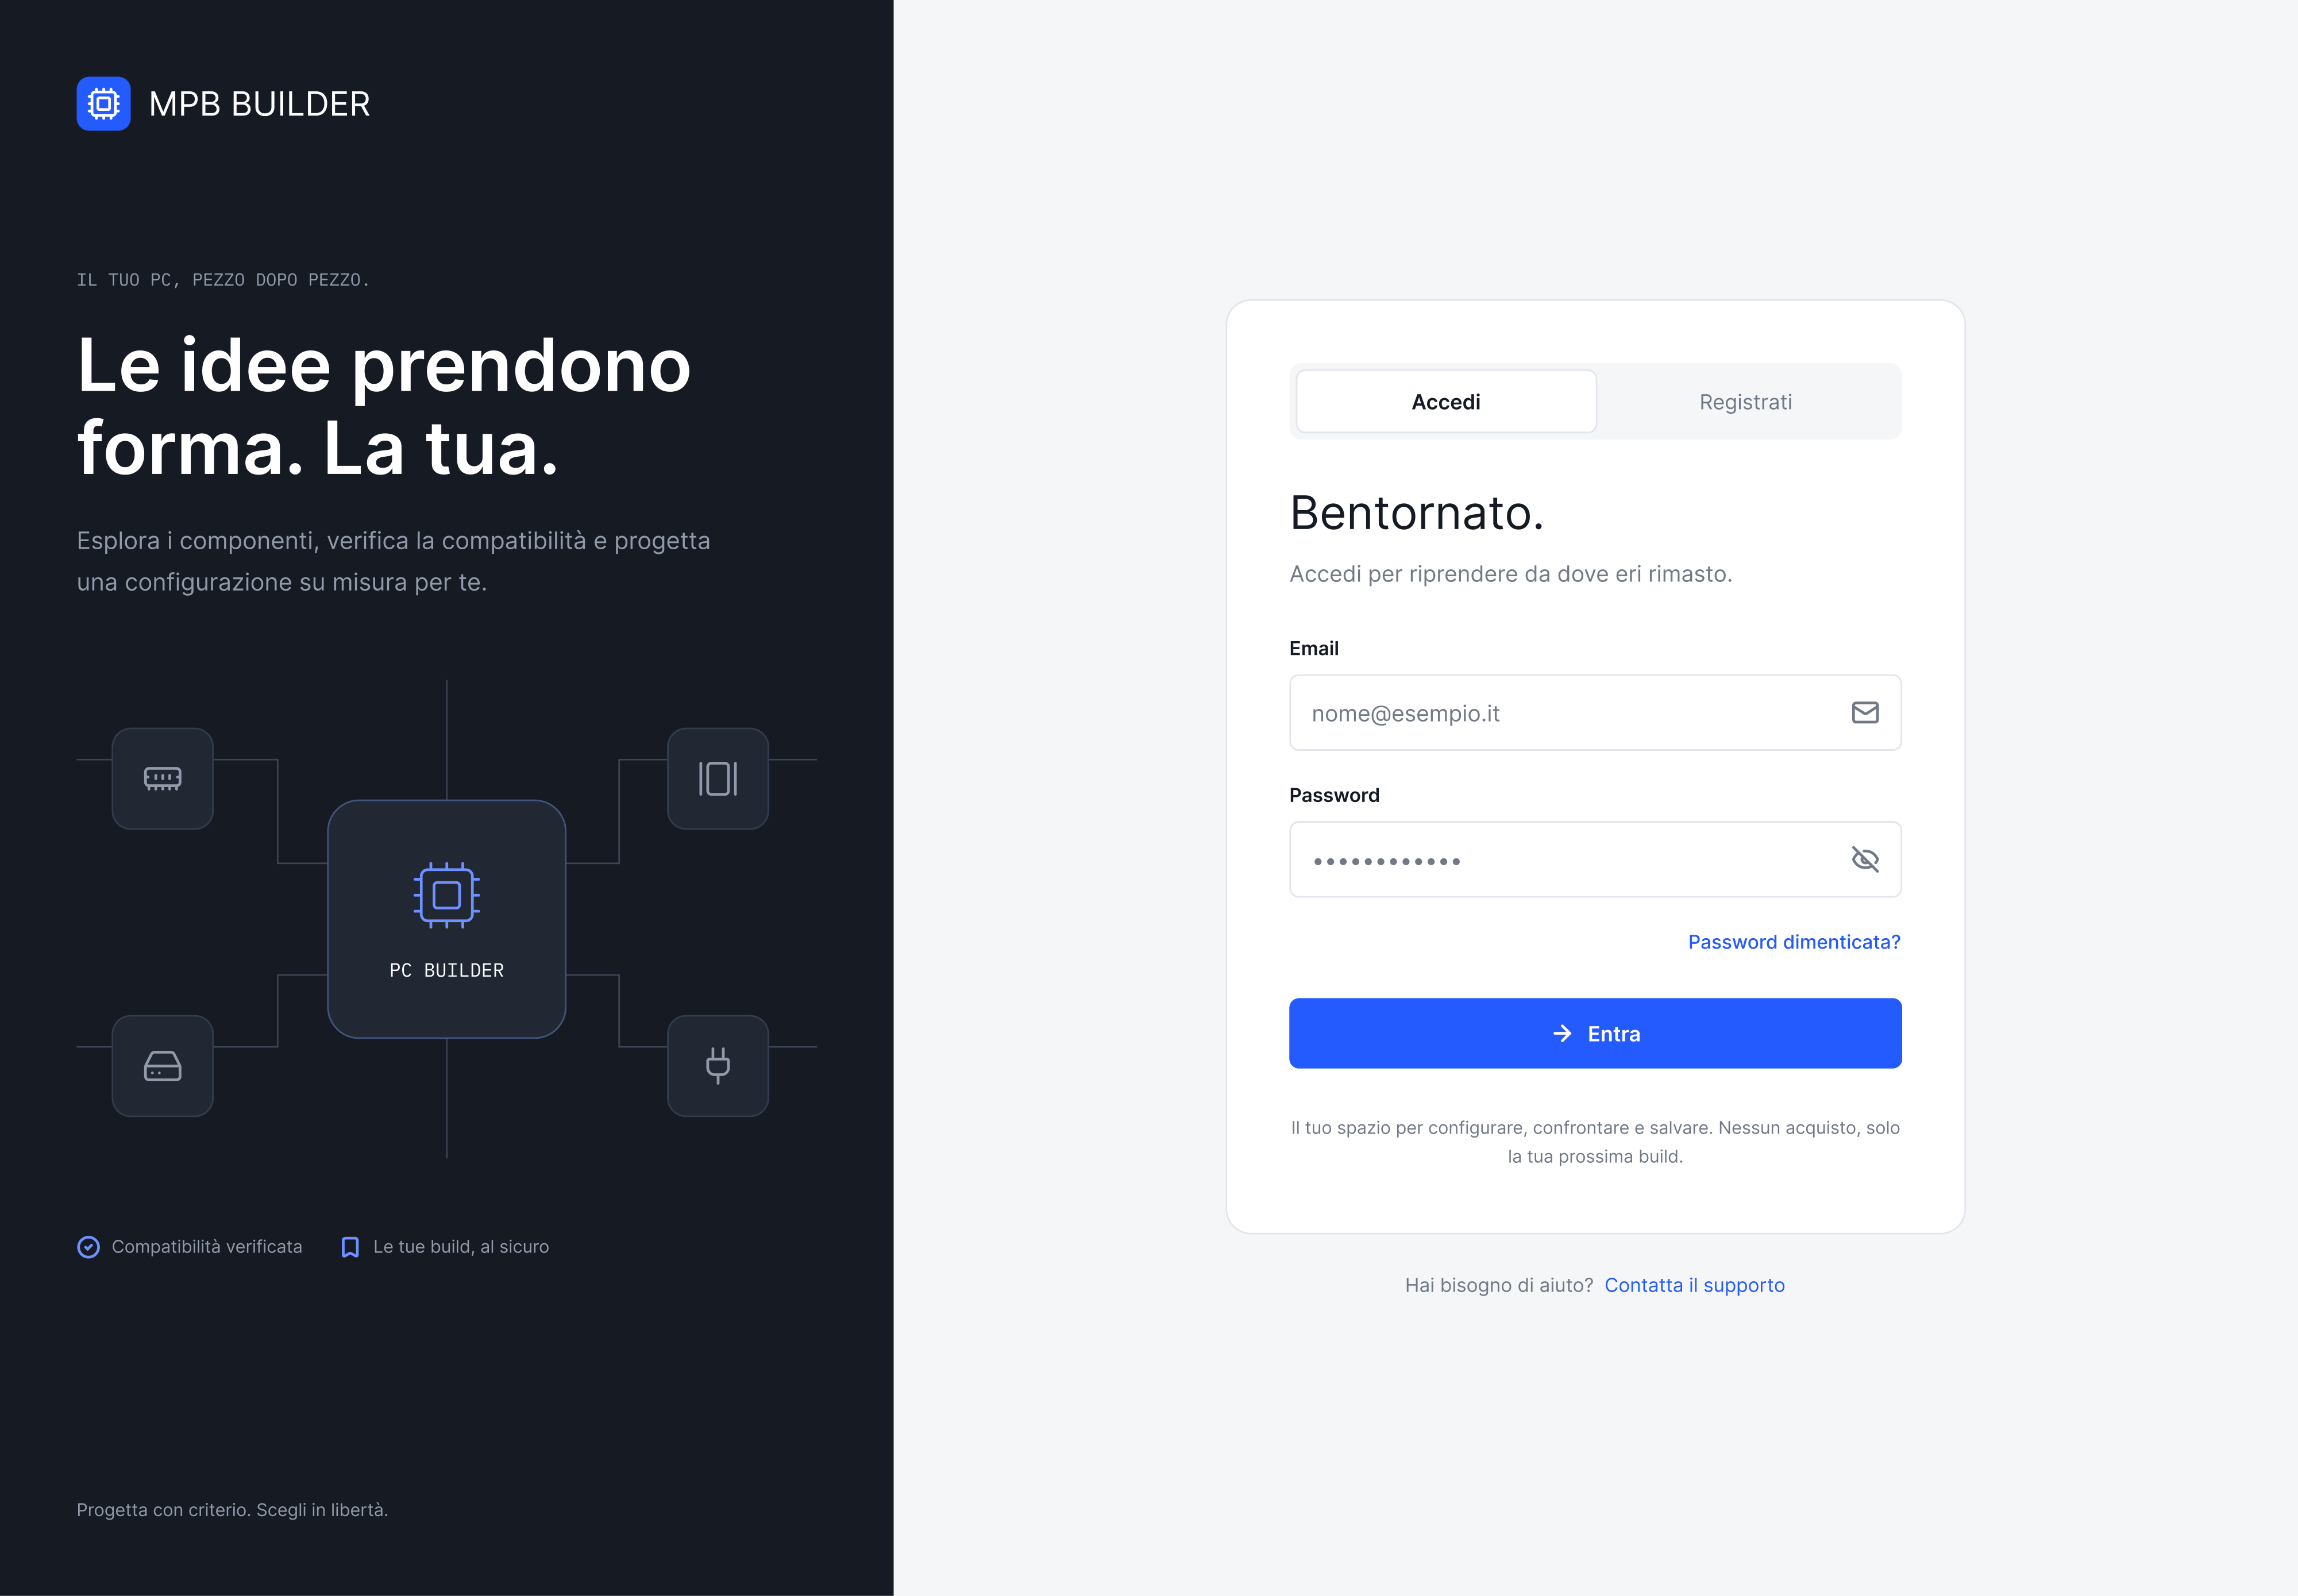
\includegraphics[width=\linewidth]{mockups/Untitled (3)-1.png}
        \caption{Mockup 1}
    \end{subfigure}\hfill
    \begin{subfigure}[t]{0.48\textwidth}
        \centering
        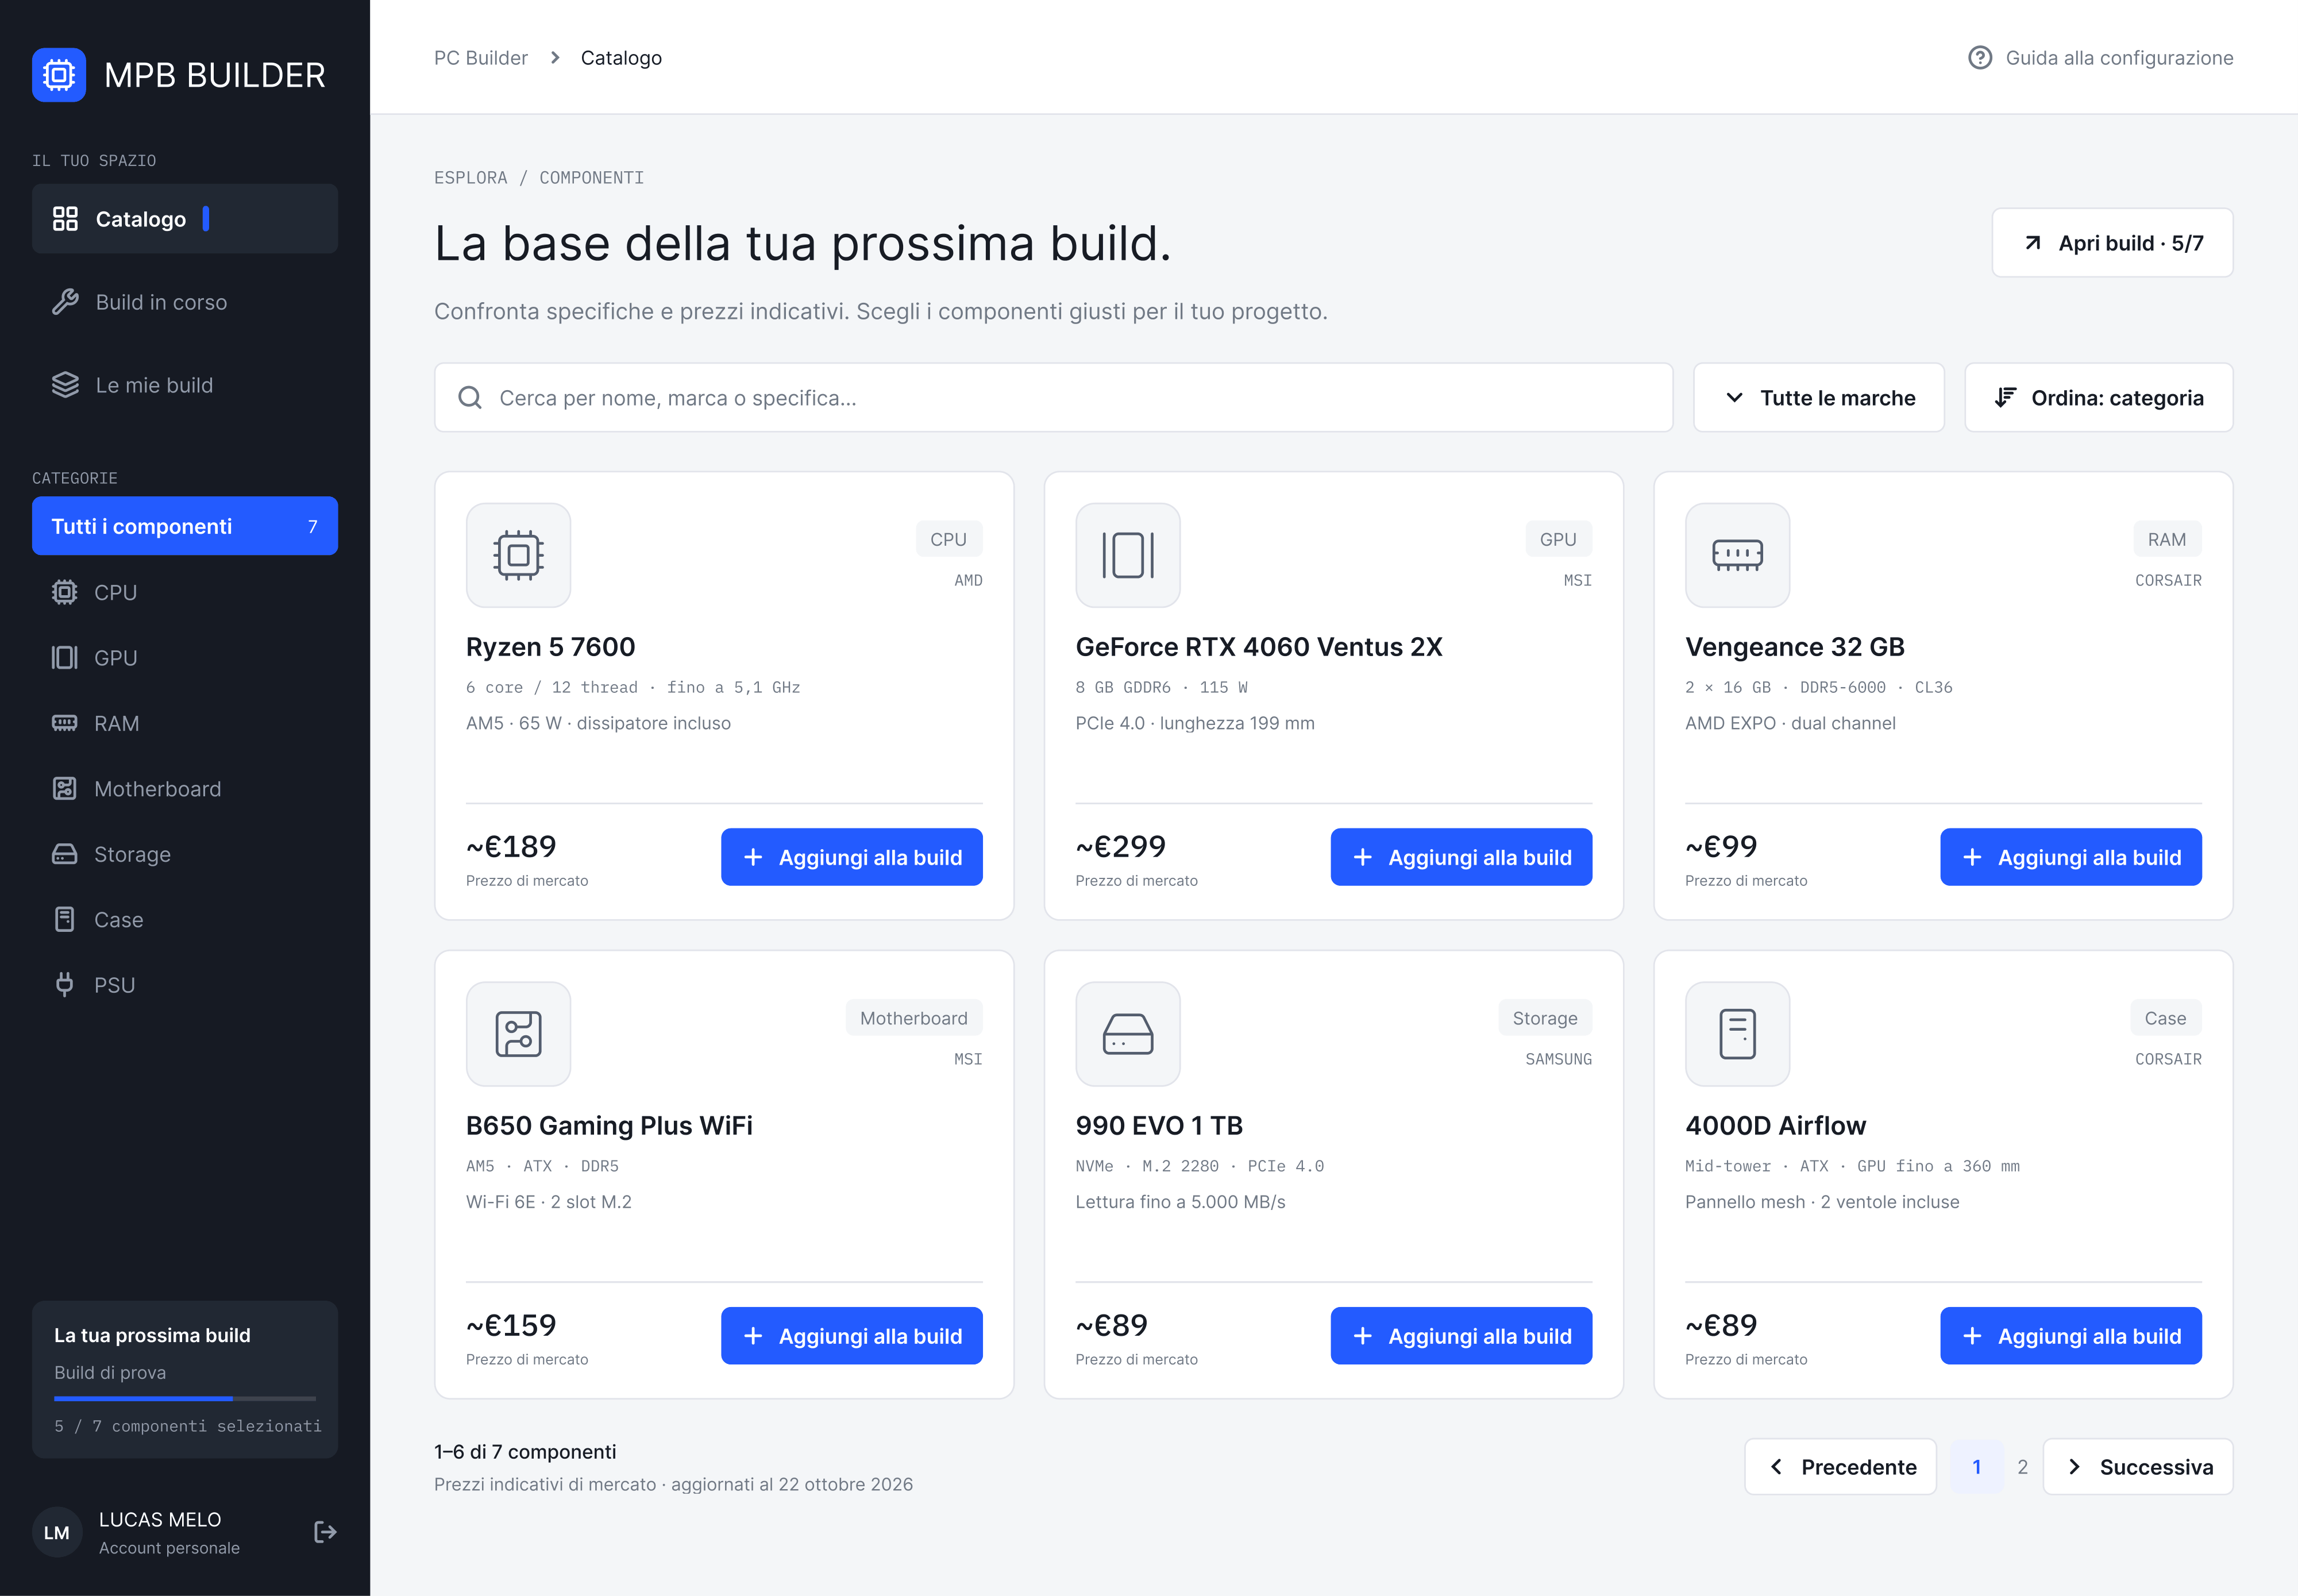
\includegraphics[width=\linewidth]{mockups/Untitled (3)-2.png}
        \caption{Mockup 2}
    \end{subfigure}

    \vspace{0.5cm}

    \begin{subfigure}[t]{0.48\textwidth}
        \centering
        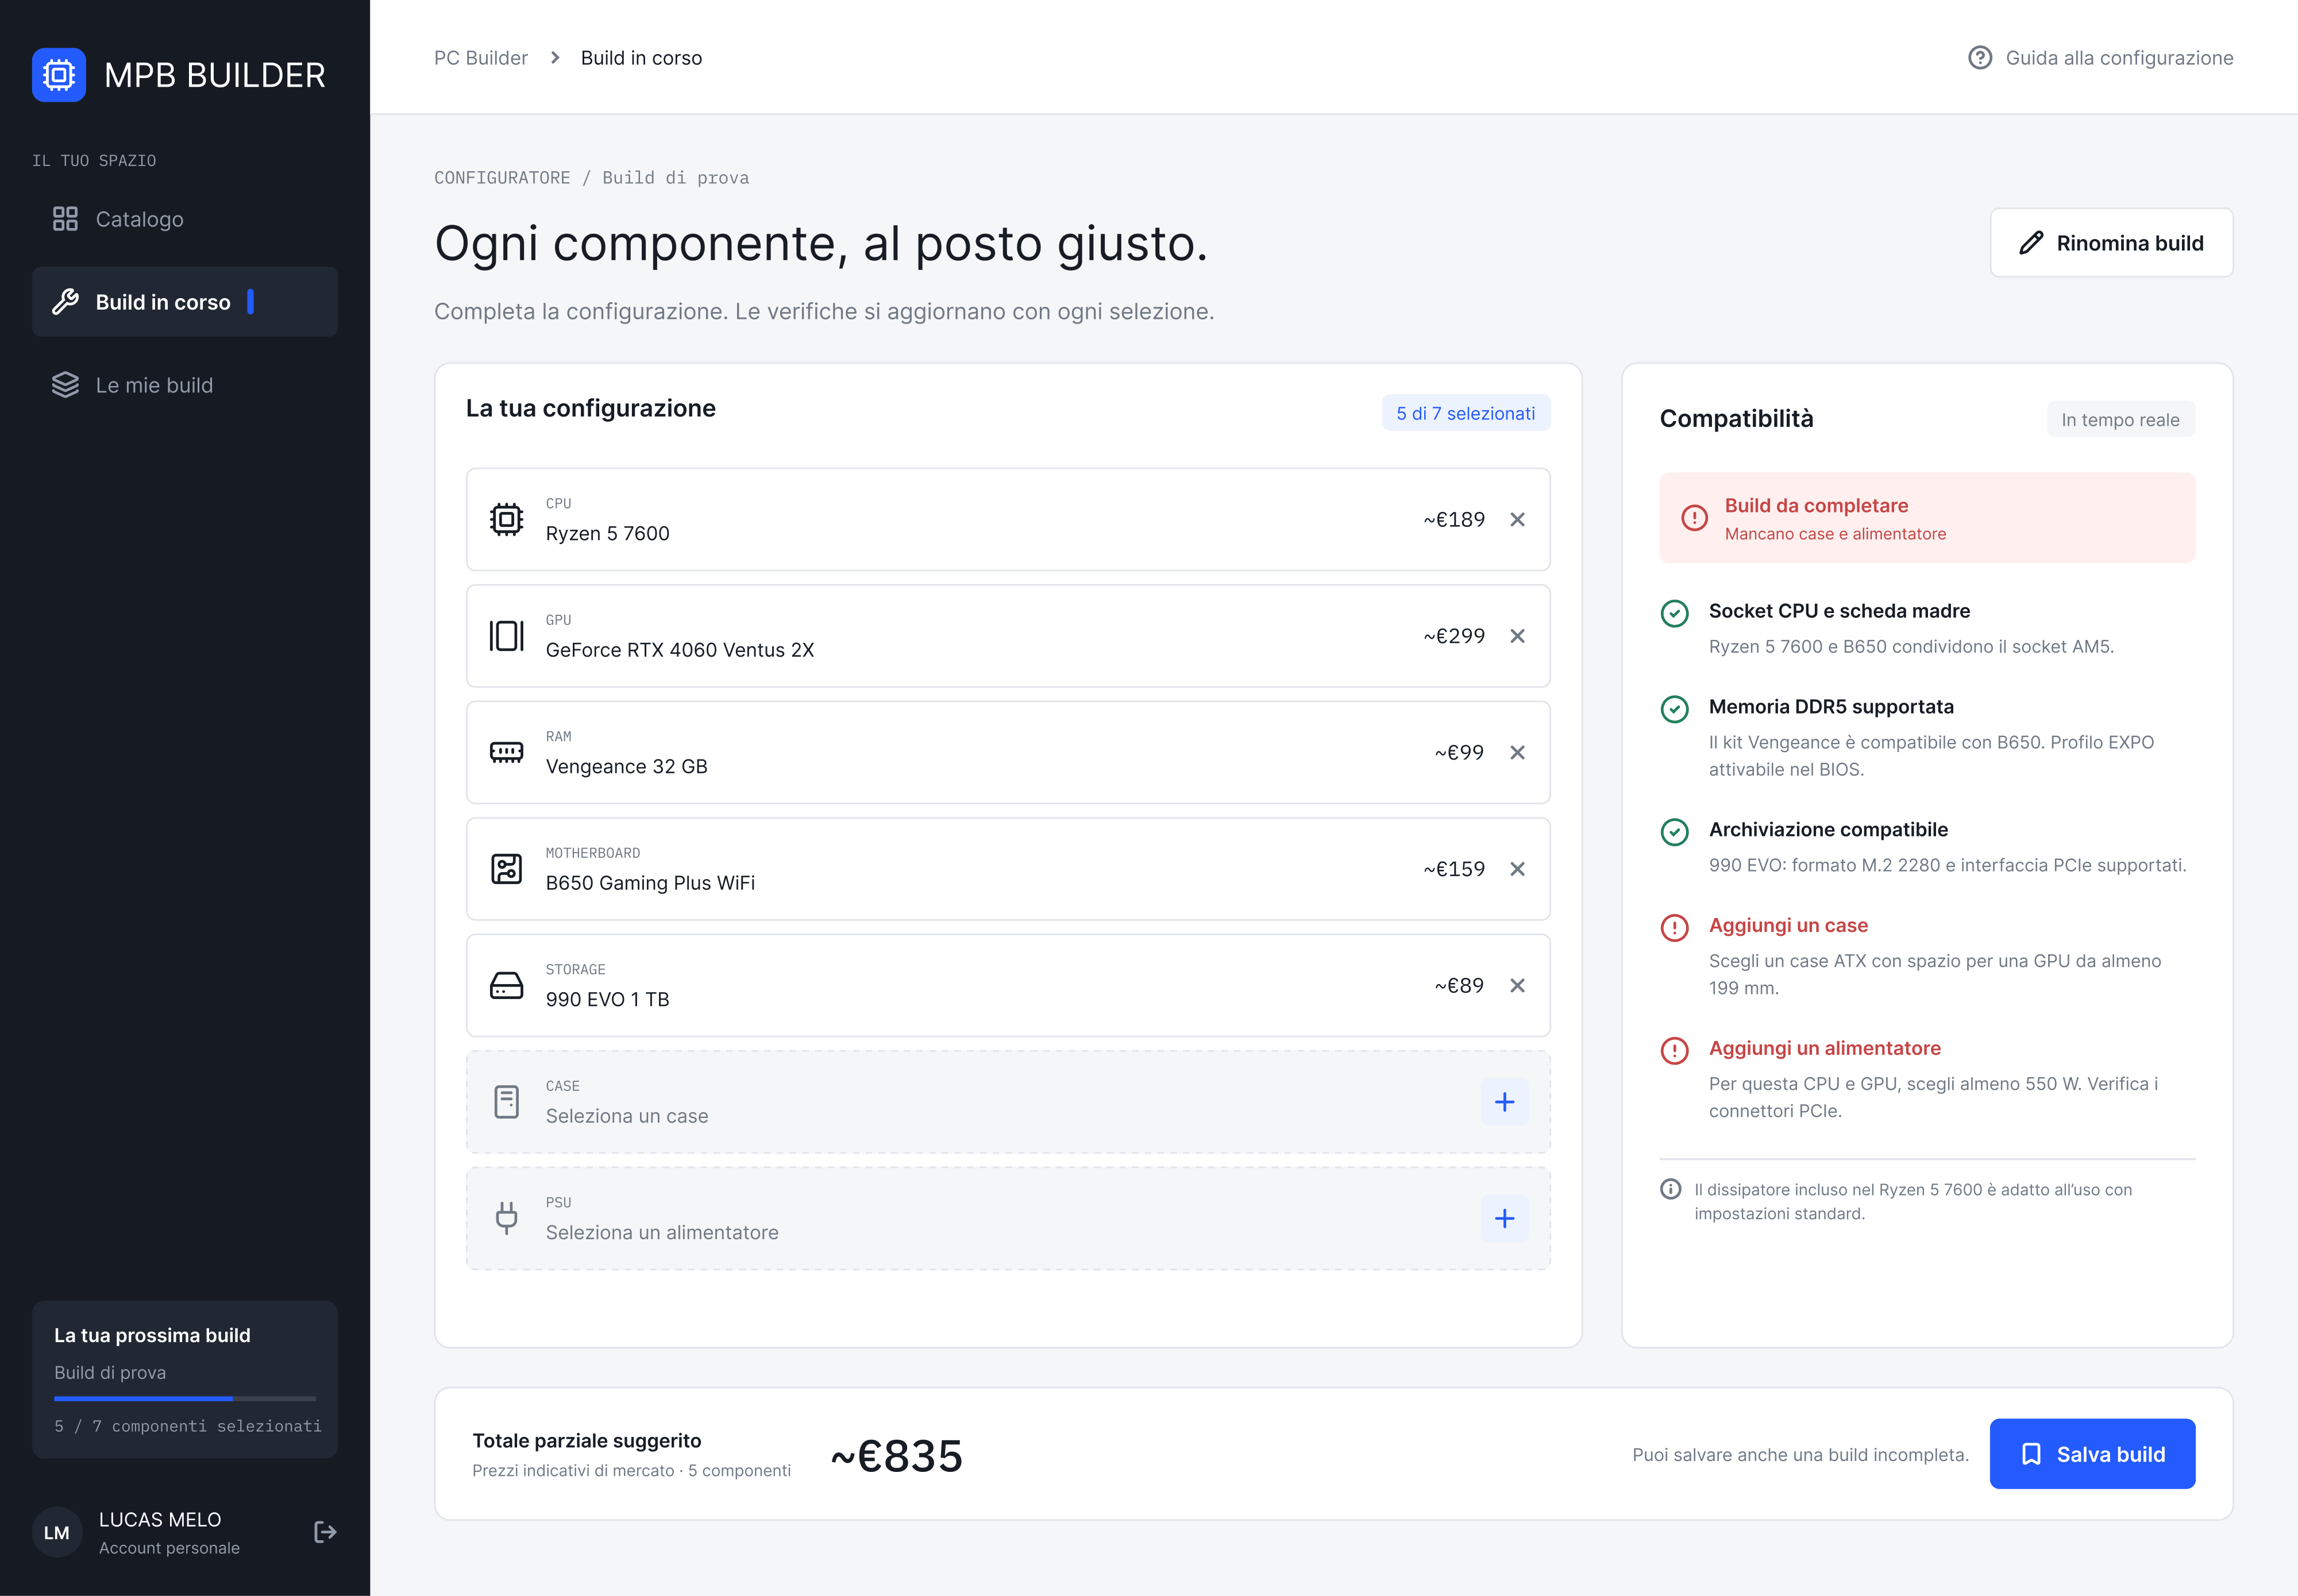
\includegraphics[width=\linewidth]{mockups/Untitled (3)-3.png}
        \caption{Mockup 3}
    \end{subfigure}\hfill
    \begin{subfigure}[t]{0.48\textwidth}
        \centering
        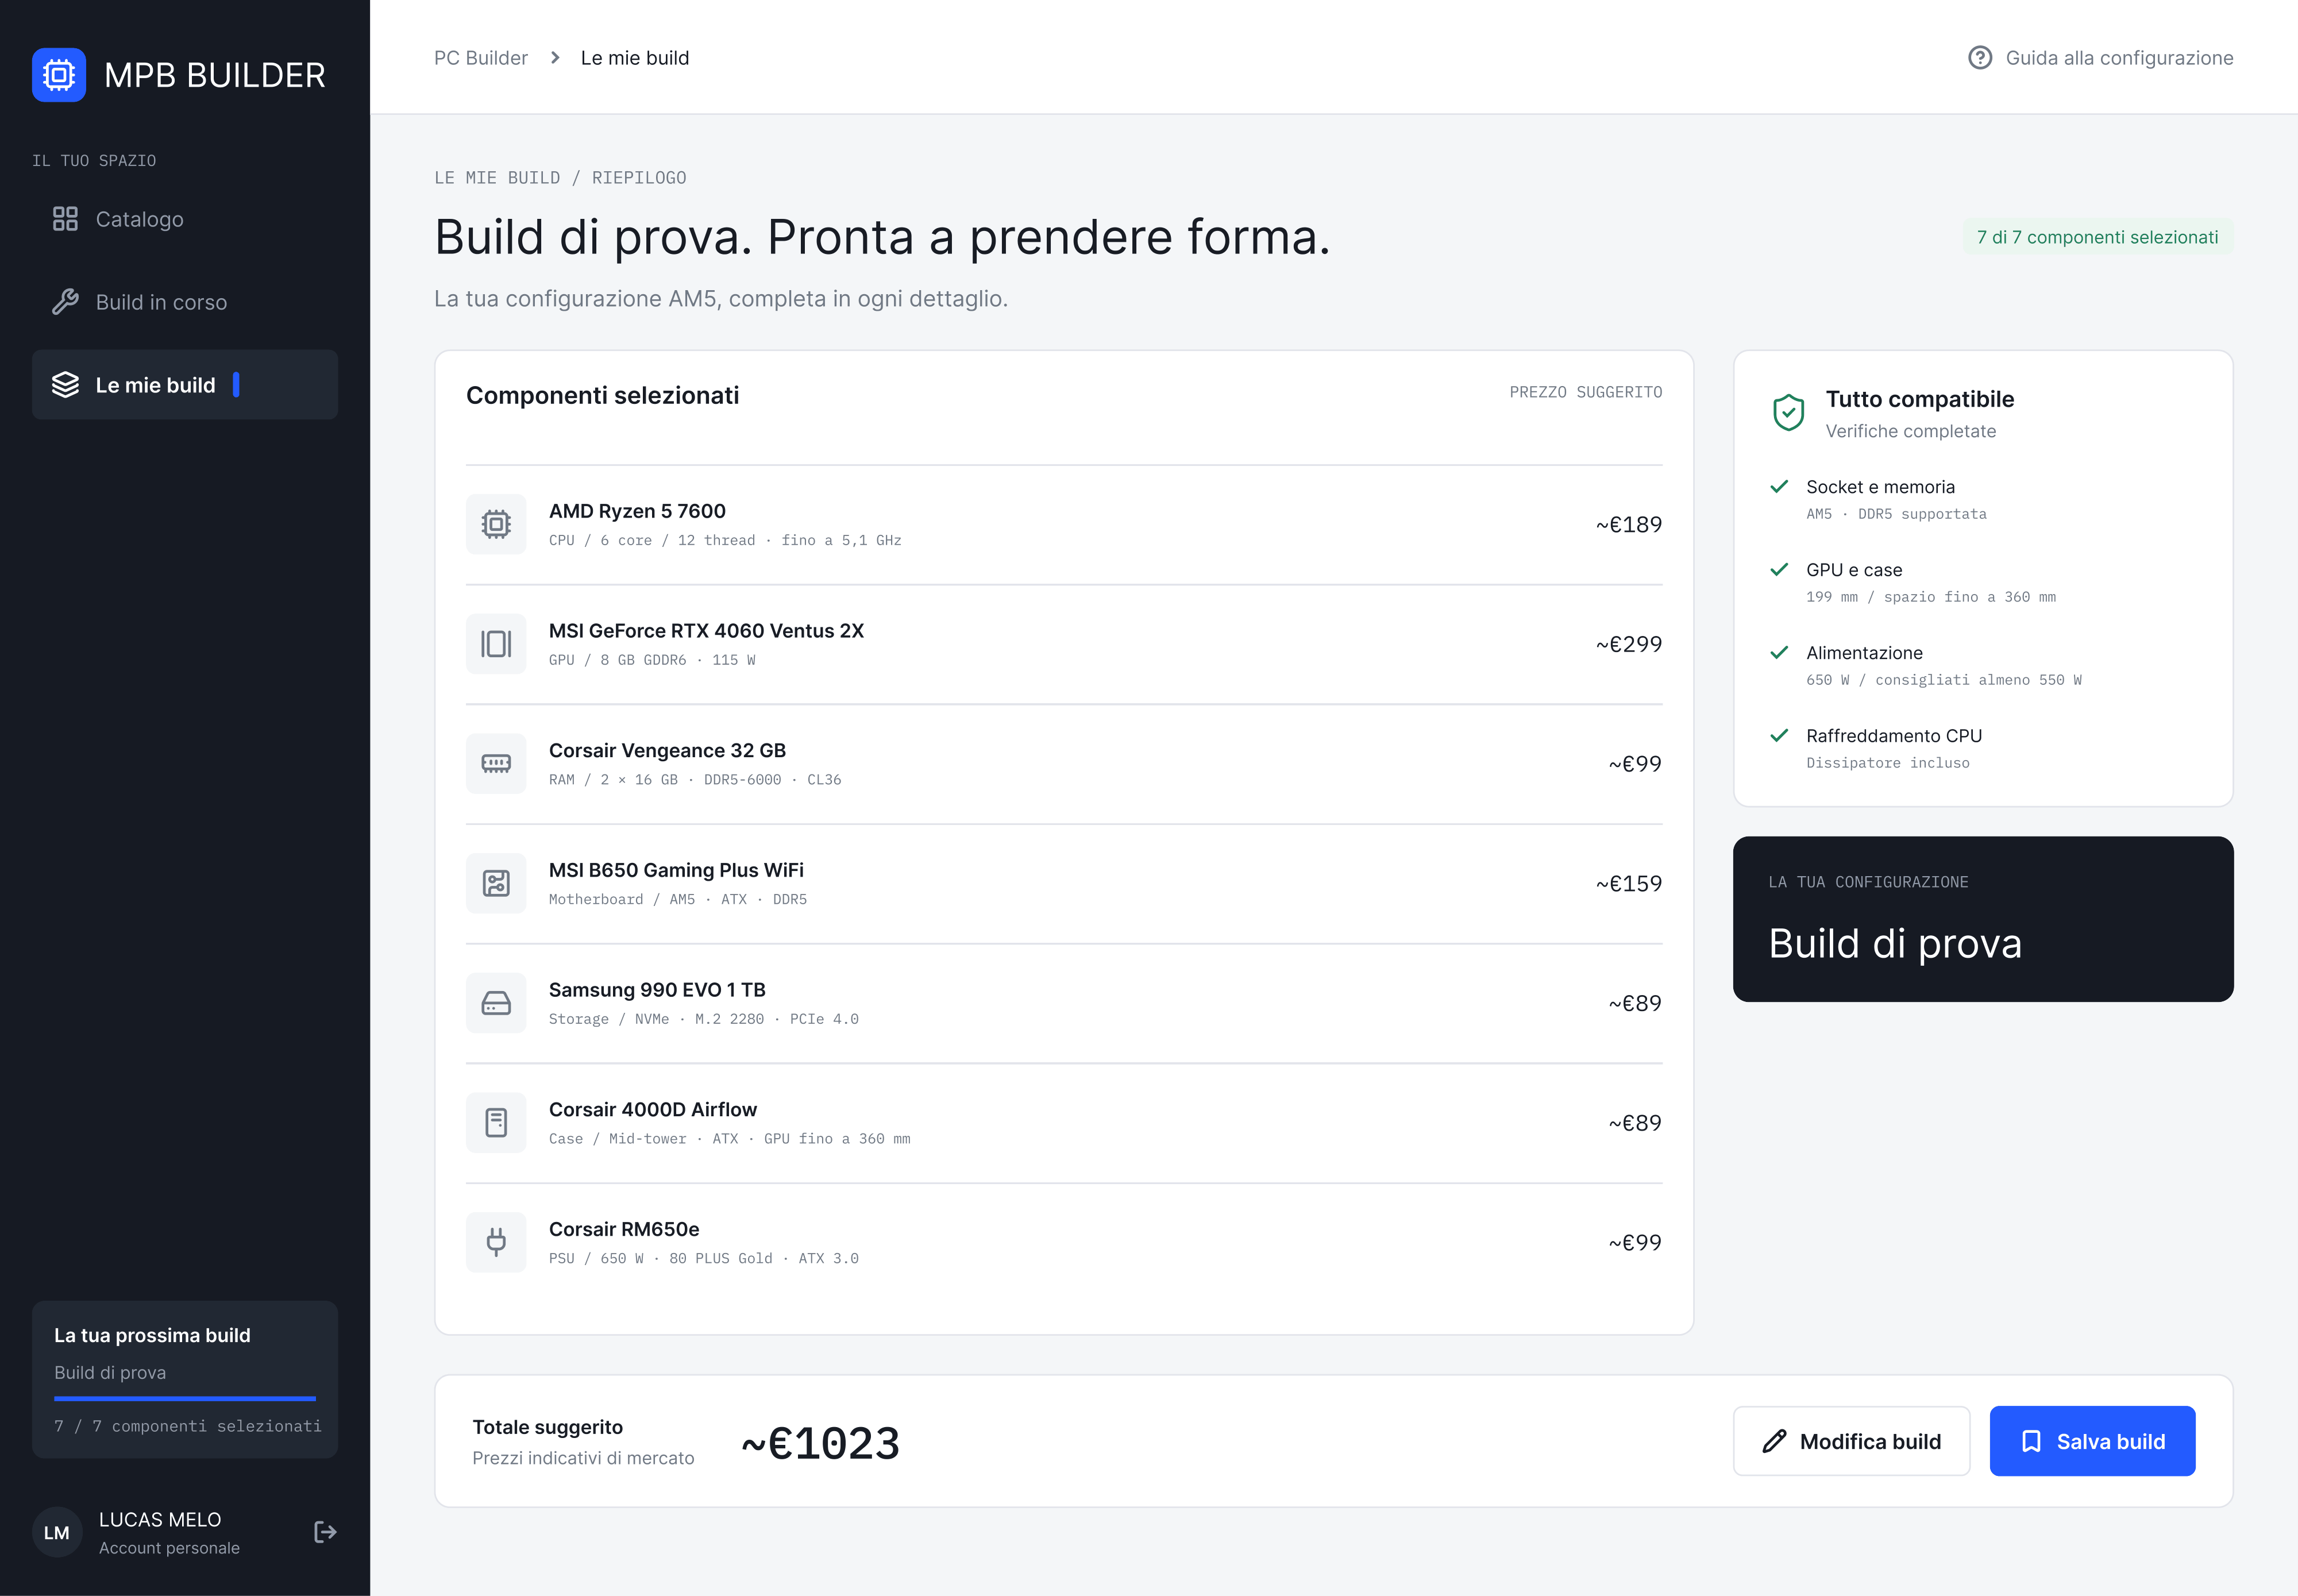
\includegraphics[width=\linewidth]{mockups/Untitled (3)-4.png}
        \caption{Mockup 4}
    \end{subfigure}

    \vspace{0.5cm}

    \begin{subfigure}[t]{0.48\textwidth}
        \centering
        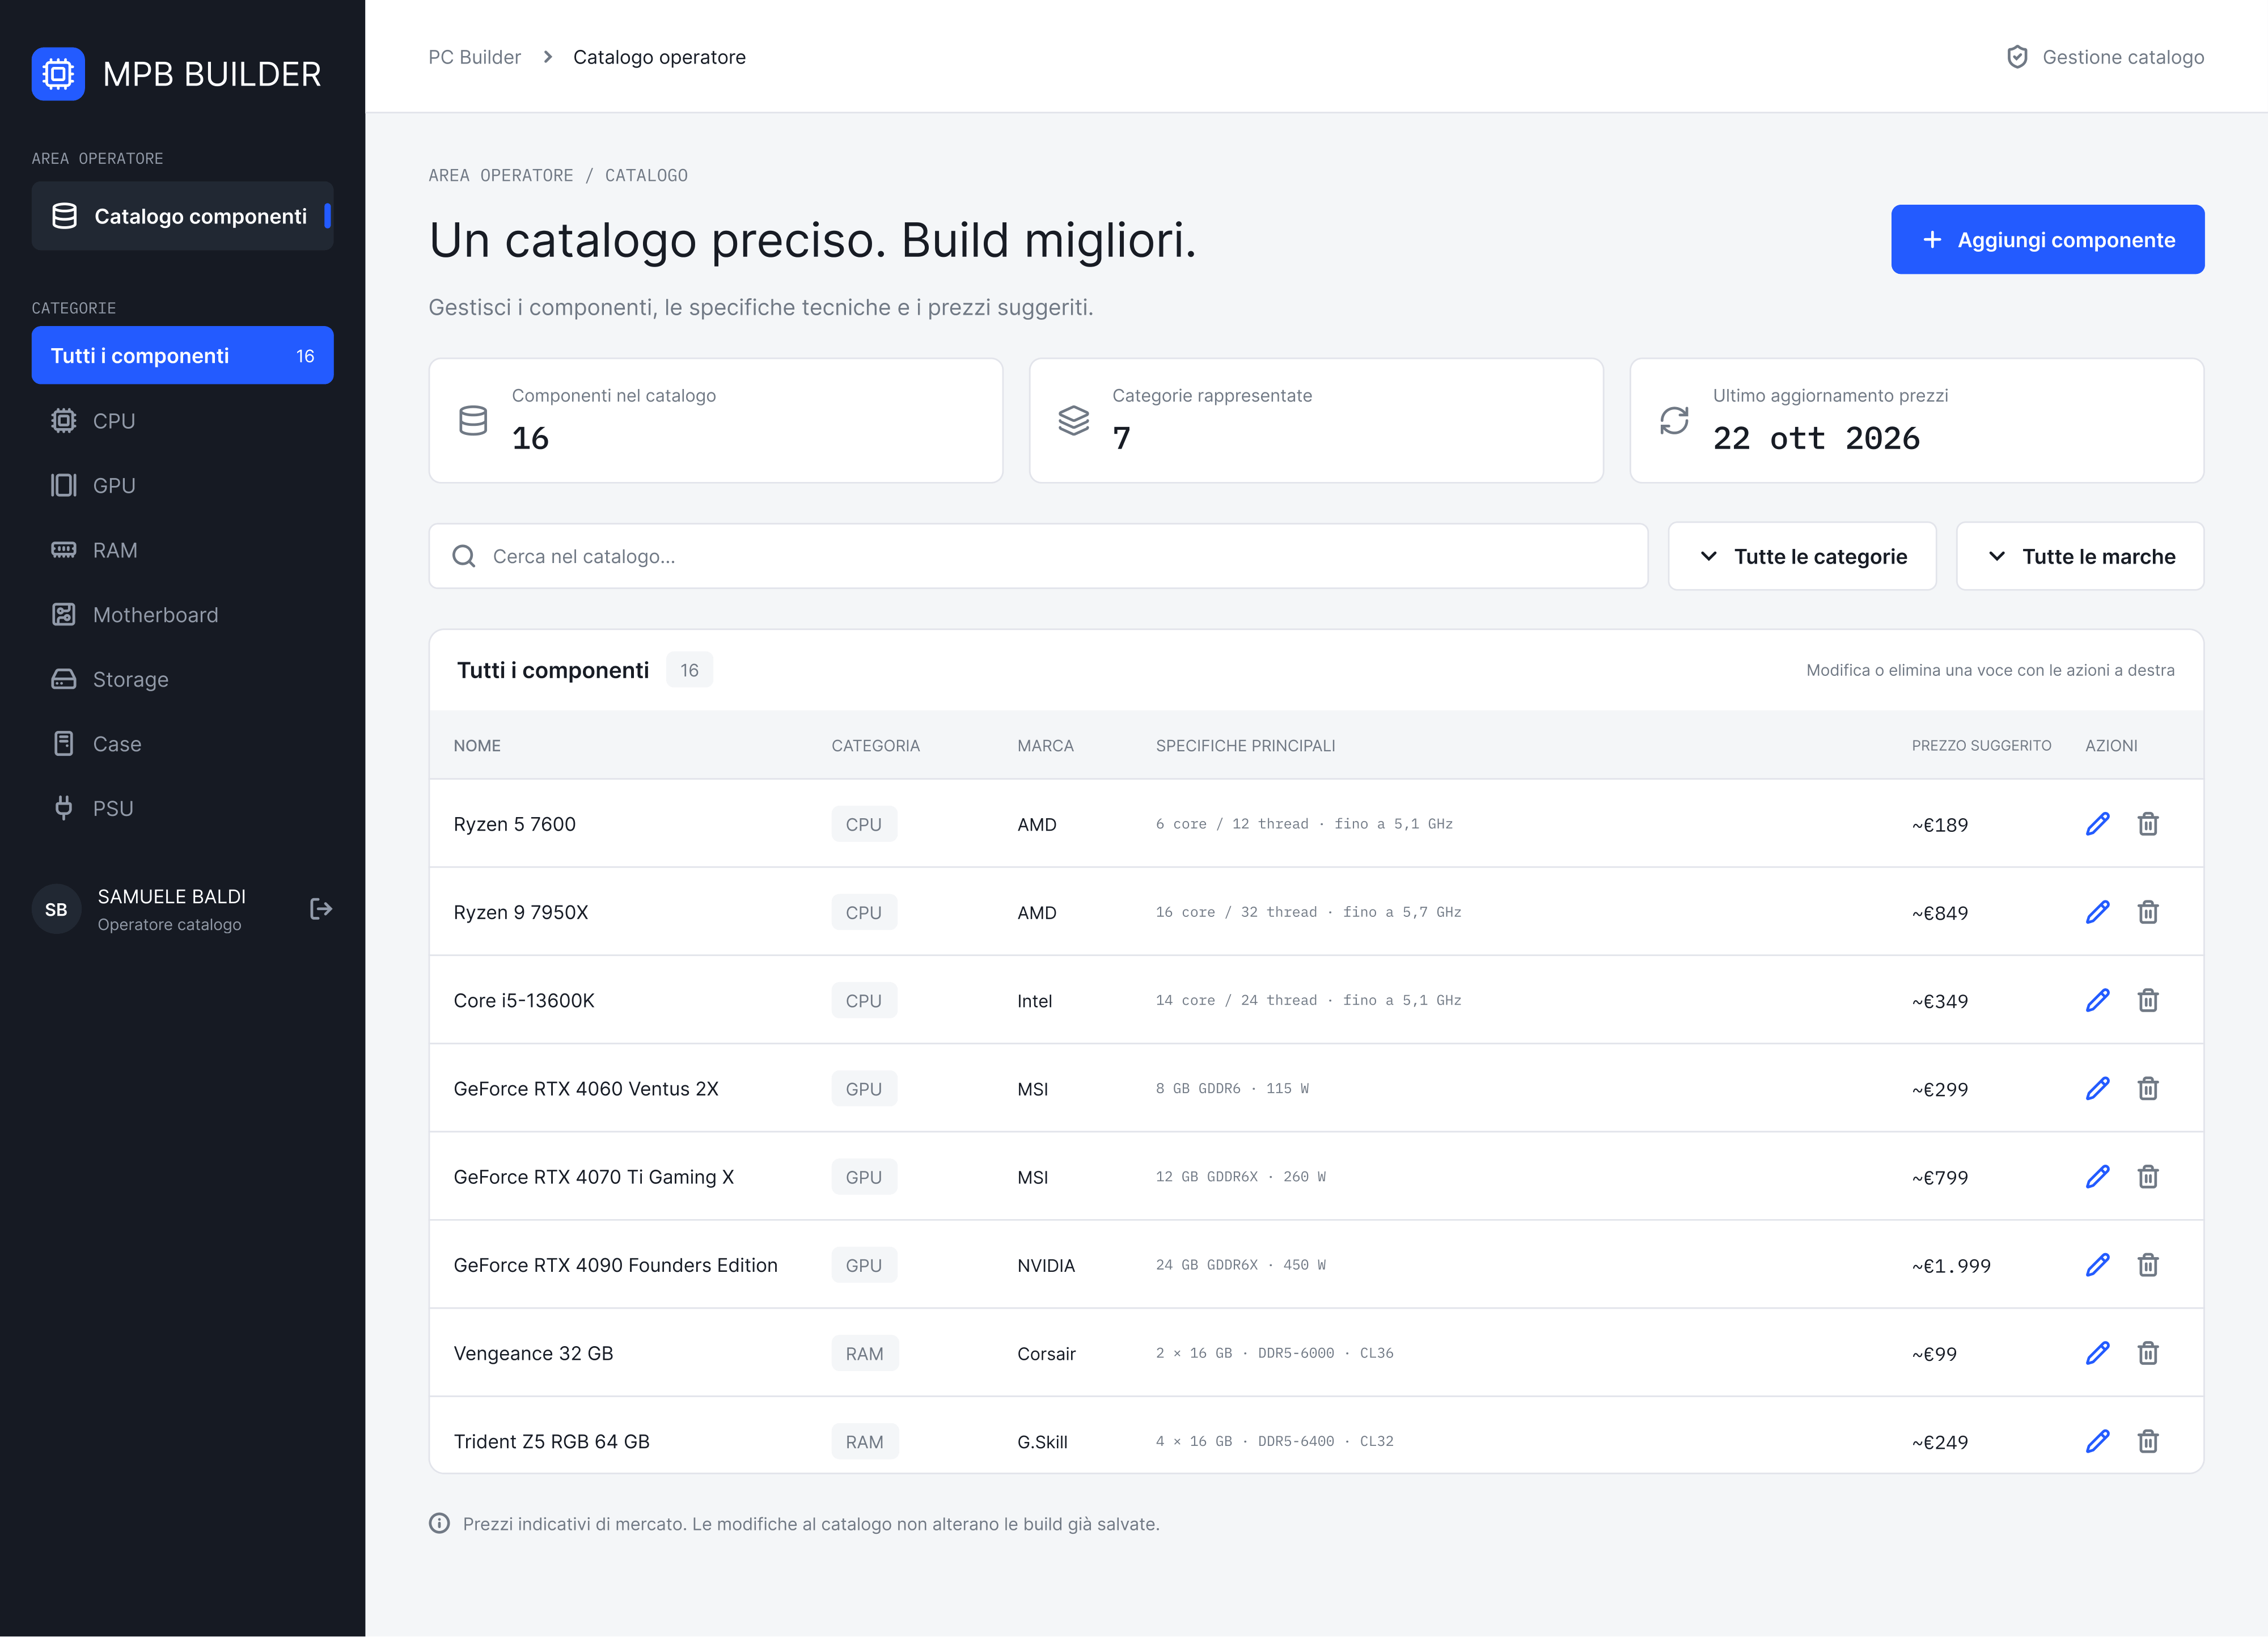
\includegraphics[width=\linewidth]{mockups/Untitled (3)-5.png}
        \caption{Mockup 5}
    \end{subfigure}
    \caption{Mockup dell'interfaccia}
    \label{fig:mockups}
\end{figure}

\subsection{Navigation Diagram}
da fare
\subsection{Class Diagram}
\begin{figure}[H]
    \centering
    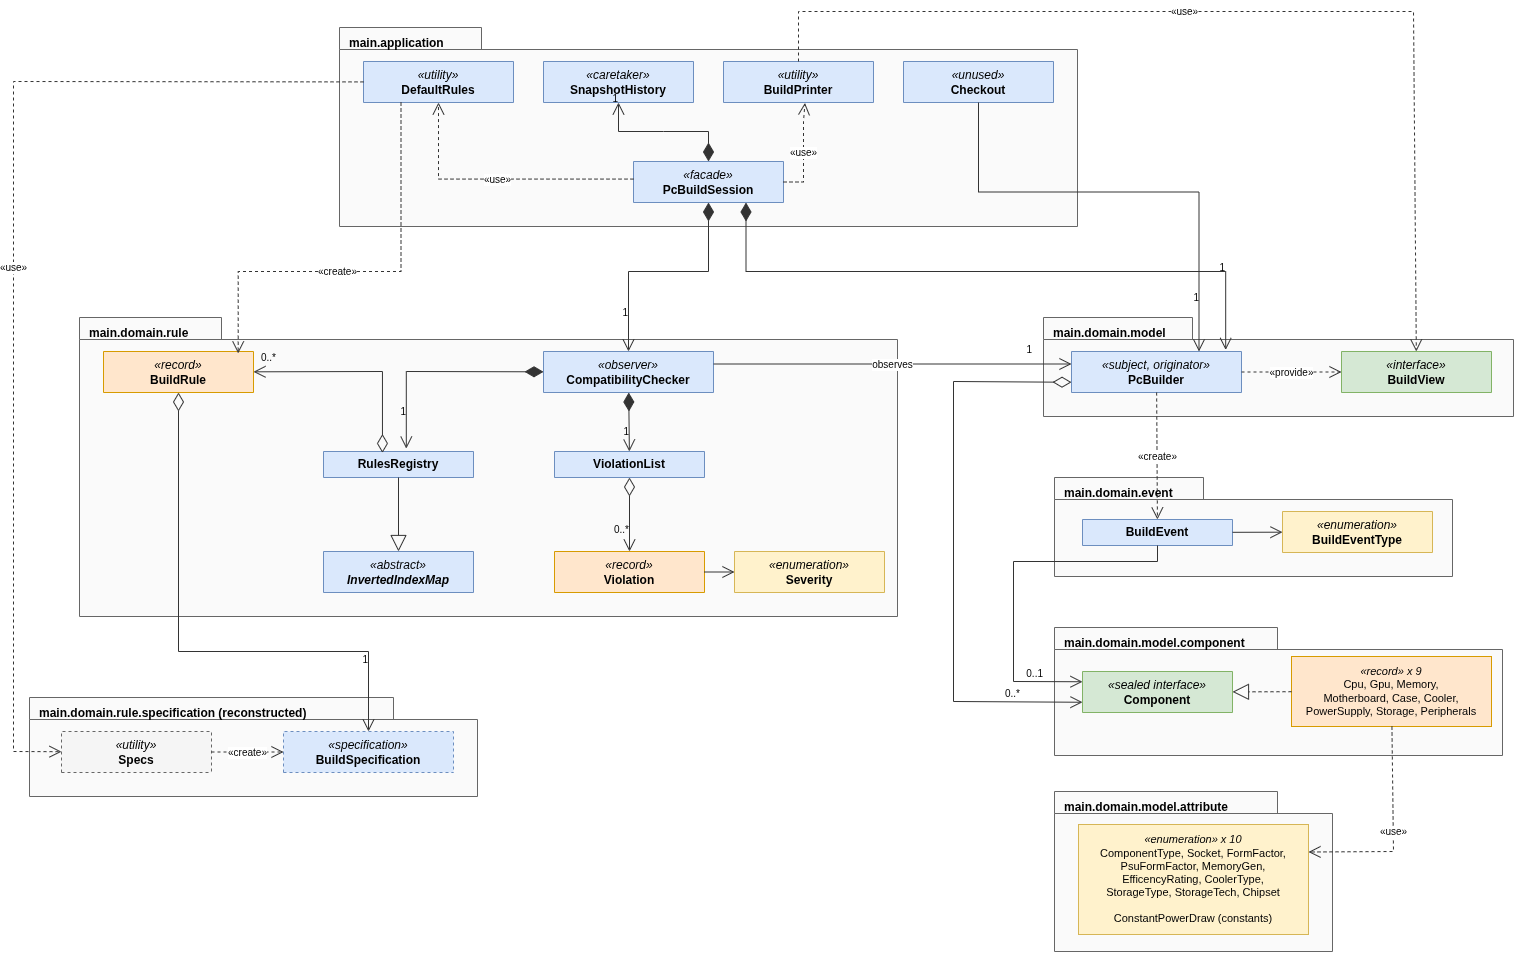
\includegraphics[width=1\linewidth]{diagrammi/overview.png}
    \caption{Enter Caption}
    \label{fig:placeholder}
\end{figure}
\subsection{ER Diagram e Modello Relazionale}
deve farla il baldè

\section{Implementazione}
\subsection{Domain}

\begin{figure}[H]
    \centering
    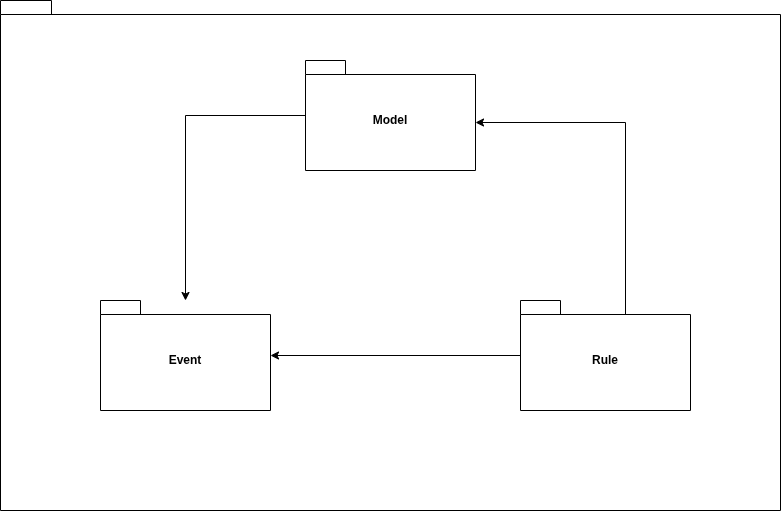
\includegraphics[width=0.5\linewidth]{diagrammi/domainpackage.png}
    \caption{Domain Package Diagram}
    \label{fig:placeholder}
\end{figure}
Il dominio contiene sia il modello che le sue business rule, nei corrispettivi pacchetti .\textit{model} e \textit{rule}

\subsubsection{Model}

\begin{figure}[H]
    \centering
    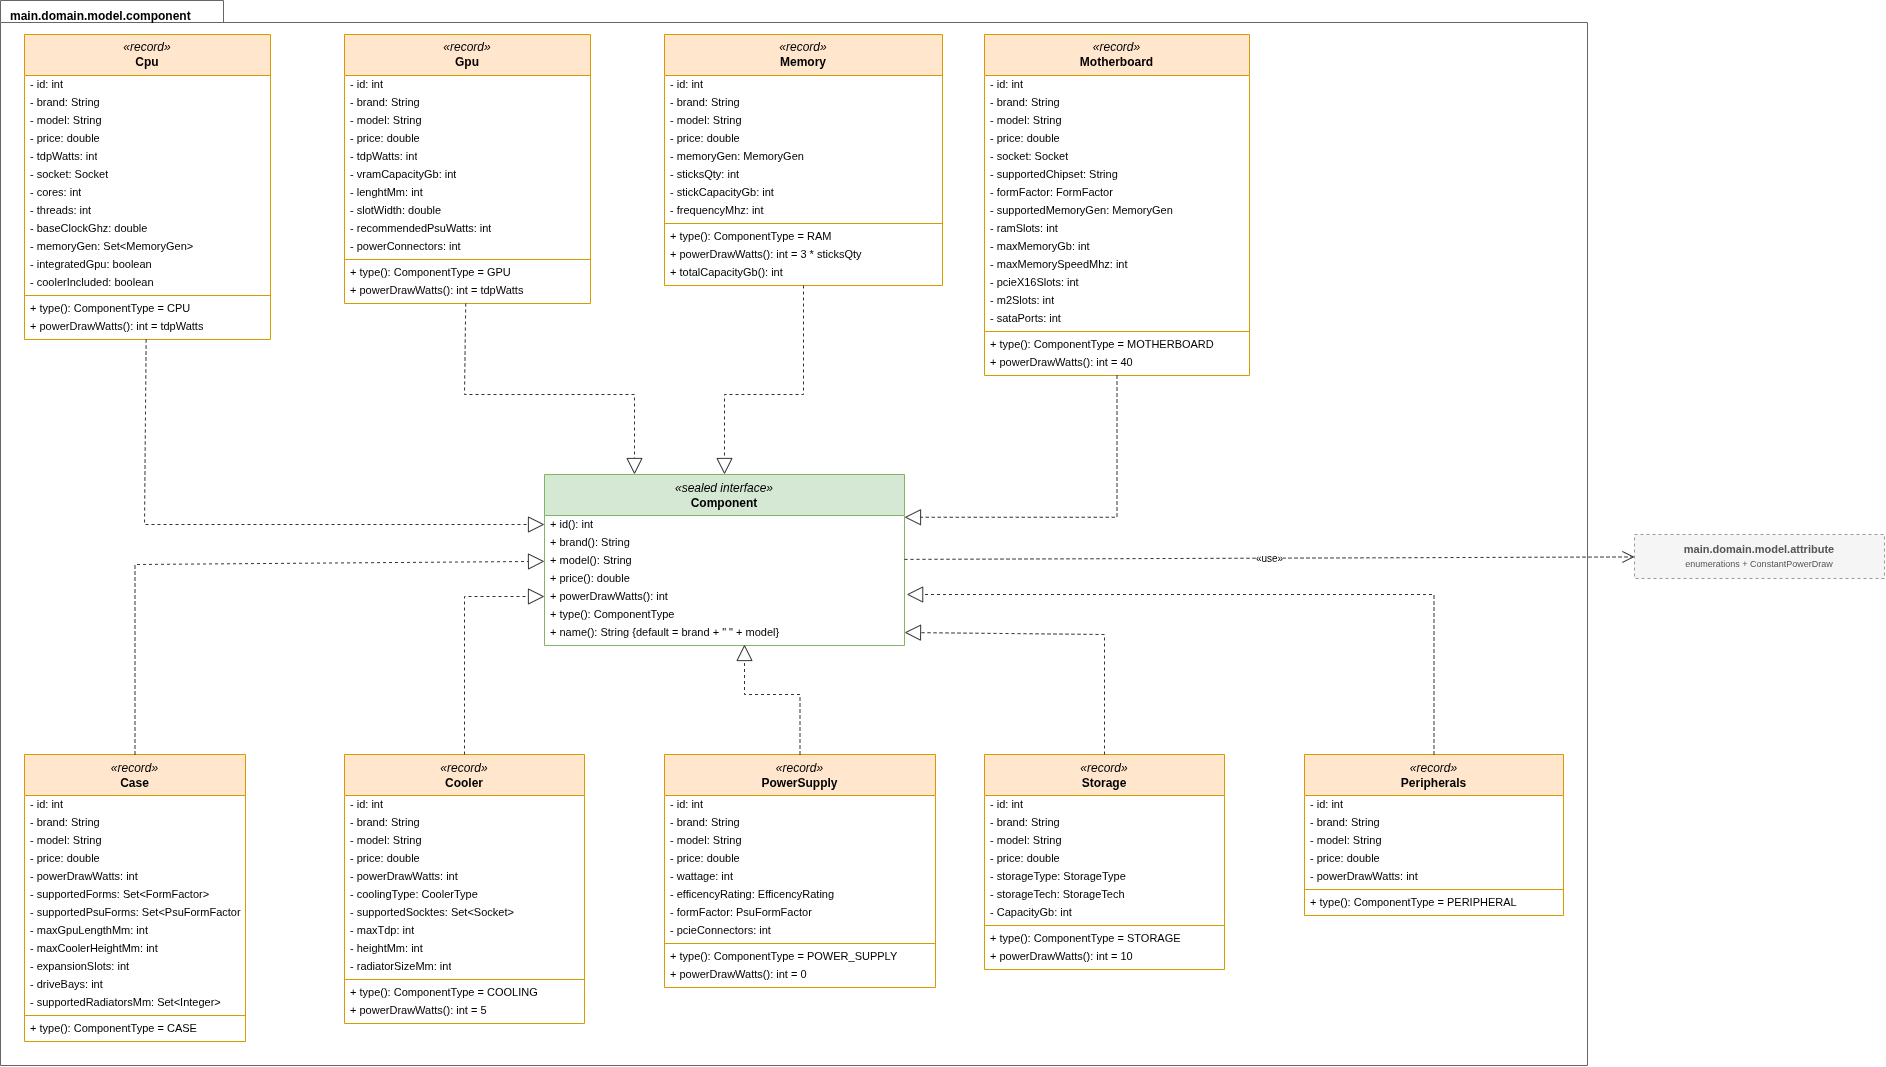
\includegraphics[width=1\linewidth]{diagrammi/Model.component.png}
    \caption{Enter Caption}
    \label{fig:placeholder}
\end{figure}

\begin{figure}[H]
    \centering
    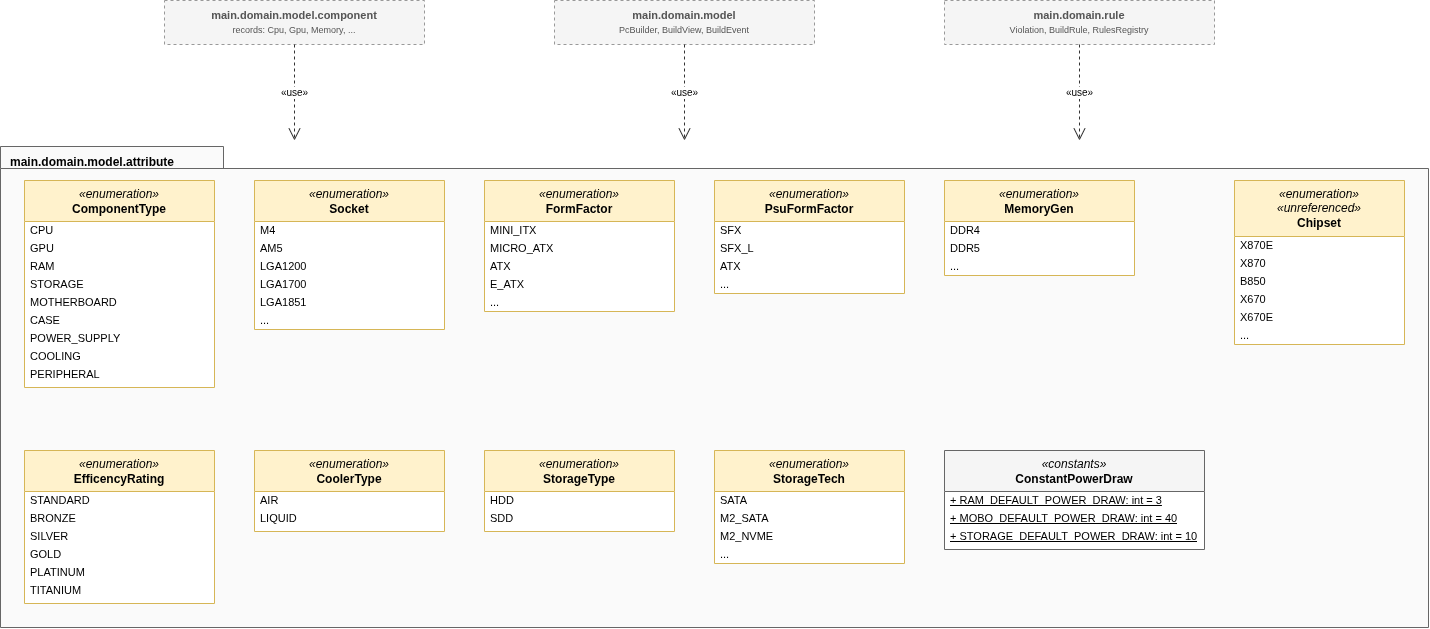
\includegraphics[width=1\linewidth]{diagrammi/model.attribute.png}
    \caption{Enter Caption}
    \label{fig:placeholder}
\end{figure}

Il modello è composto da due sottopacchetti:
\begin{itemize}
    \item \textbf{component} contiene l'interfaccia chiusa \textit{Component}, che viene implementata dalle tipologie possibili tipologie di componenti come \textit{record}. La scelta di implementarli come record deriva dalla loro natura costante e immutabile della collezione di informazioni che rappresenta ogni componente, perciò è possibile sfruttare la sintassi più semplice e i vantaggi per la jvm.\\

\begin{lstlisting}[style=intellijlight, caption={A simple Java class}, label={lst:hello}]
//Component.java
package main.domain.model.component;

public sealed interface Component
        permits Case, Gpu, Peripherals, Cooler, Cpu, 
        Memory, Motherboard, PowerSupply, Storage {

    int id();
    String brand();
    String model();
    double price();

    int powerDrawWatts();

    public ComponentType type();
    default String name() { return brand() + " " + model(); }

}
\end{lstlisting}
    
    
    I record in questione sono i seguenti:
    \begin{itemize}
        \item \texttt{Cpu}
        \item \texttt{Gpu}
        \item \texttt{Motherboard}
        \item \texttt{Memory}
        \item \texttt{Storage}
        \item \texttt{Case}
        \item \texttt{PowerSupply}
        \item \texttt{Peripherals}
    \end{itemize}
    
    
\end{itemize}
\begin{itemize}
\item \textbf{attribute} contiene invece le enumerazioni che determinano le tipologie le caratteristiche dei componenti. queste sono:
\begin{itemize}
\item \texttt{ComponentType}
\item \texttt{Chipset}
\item \texttt{CoolerType}
\item \texttt{EfficencyRating}
\item \texttt{FormFactor}
\item \texttt{MemoryGen}
\item \texttt{PsuFormFactor}
\item \texttt{Socket}
\item \texttt{StorageTech}
\item \texttt{StorageType}
\item \texttt{ConstantPowerDraw} (non è un'enum a differenza degli altri)
\end{itemize}
\end{itemize}

\begin{lstlisting}[style=intellijlight, caption={A simple Java class}, label={lst:hello}]
//ComponentType.java
package main.domain.model.attribute;

public enum ComponentType {
    CPU,
    GPU,
    RAM,
    STORAGE,
    MOTHERBOARD,
    CASE,
    POWER_SUPPLY,
    COOLING,
    PERIPHERAL
}
\end{lstlisting}

Tutti questi componenti verranno poi composti tra di loro per ottenere la build completa del pc, che rappresenta il punto centrale dell'applicazione. La classe che si occupa di questo è \texttt{PcBuilder}, che raccoglie tutti i componenti in un'\textit{EnumMap}: le chiavi sono quelle fornite dall'enumerazione \texttt{ComponentType}, mentre i valori sono delle liste di elementi \texttt{Component}, che contengono i componenti per a seconda della corrispettiva tipologia.\\
Le liste possono contenere più elementi per tipologia, questo però è un comportamento consentito dal metodo \texttt{addComponent()} e da \texttt{CompatibilityChecker}: un utente può inserire ad esempio due cpu alla configurazione (magari per confrontarle in un attimo di decisione), questa irregolarità verrà poi segnalata in \texttt{ViolationList} e non sarà possibile effettuare il checkout finché queste persistono.

\begin{figure}[H]
    \centering
    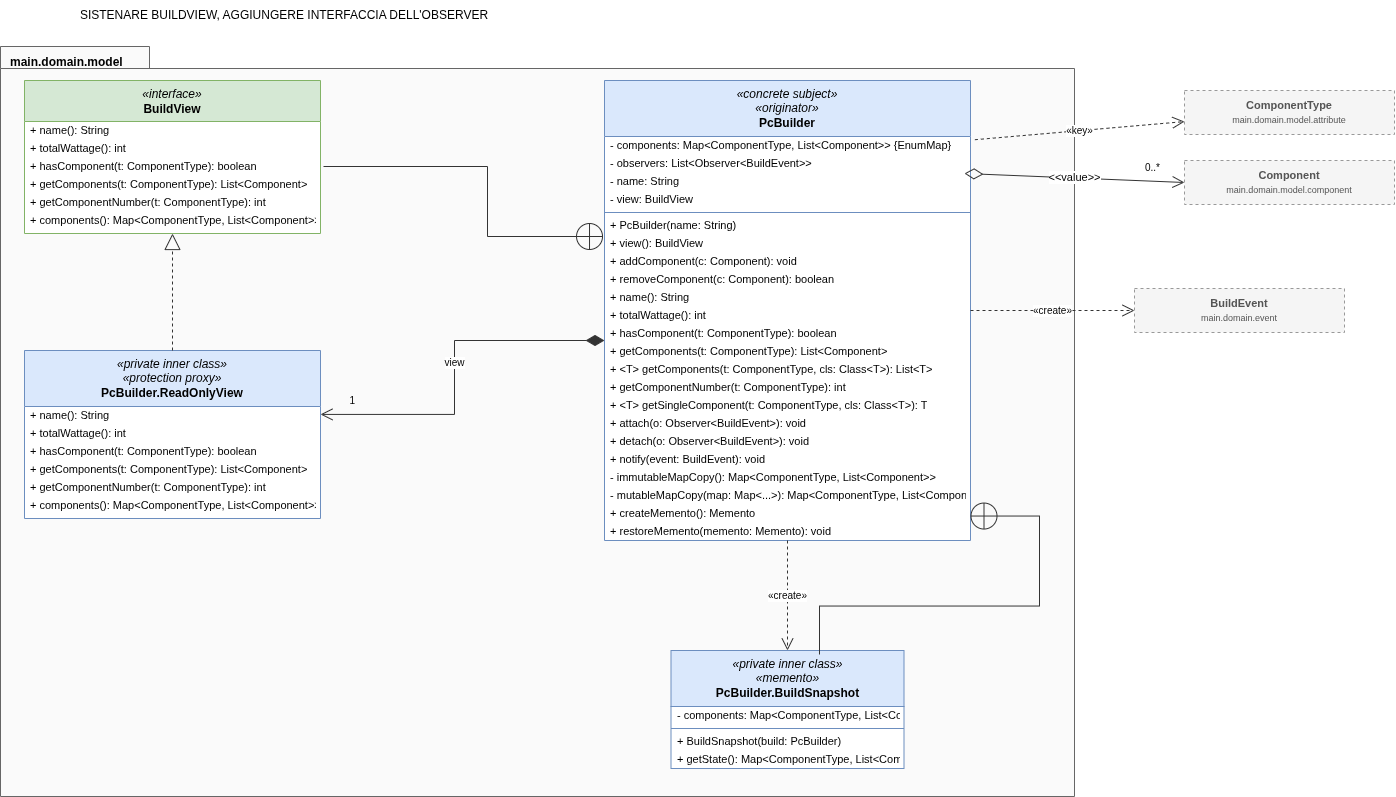
\includegraphics[width=1\linewidth]{diagrammi/model.pcbuilder.png}
    \caption{Enter Caption}
    \label{fig:placeholder}
\end{figure}

\texttt{PcBuilder} contiene al suo interno due classi astratte:
\begin{itemize}
    \item \texttt{ReadonlyView}: implementa l'interfaccia pubblica BuildView. Se questa interfaccia fosse implementata da PcBuilder direttamente, sarebbe possibile effettuare il cast \texttt{ (PcBuilder) session.getBuild()...} e violare i limiti di sola lettura imposta dall'interfaccia. Implementare invece quetsa interfaccia in una classe privata che funge da \textit{Proxy}, rende impossibile questo "escamotage".
    \item \texttt{BuildSnapshot}: permette l'implementazione corretta di memento. Questa classe privata è la migliore alternativa alla funzionalità \textit{friend} del C++ (mancante in java) utilizzata in \textit{GoF} per implementare memento: quindi BuildSnapshot implementa l'interfaccia pubblica \texttt{Memento} e il tipo che ritorna \textit{createMemento} è il medesimo, così all'esterno non è possibile effettuare un cast alla classe privata i questione preservando la segretezza dello stato del memento al di fuori di \textit{Originator}.
\end{itemize}

\subsubsection{Event}
\begin{figure}[H]
    \centering
    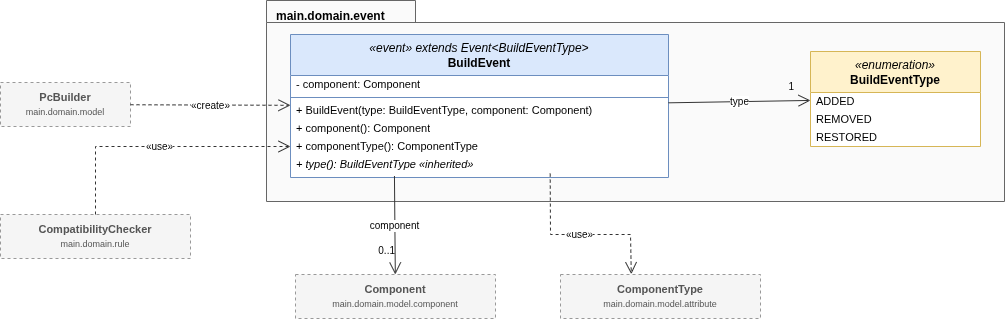
\includegraphics[width=1\linewidth]{diagrammi/model.event.png}
    \caption{Enter Caption}
    \label{fig:placeholder}
\end{figure}
Contiene le informazioni su che modifica è stata effettuata...

\subsubsection{Rule}
\begin{figure}[H]
    \centering
    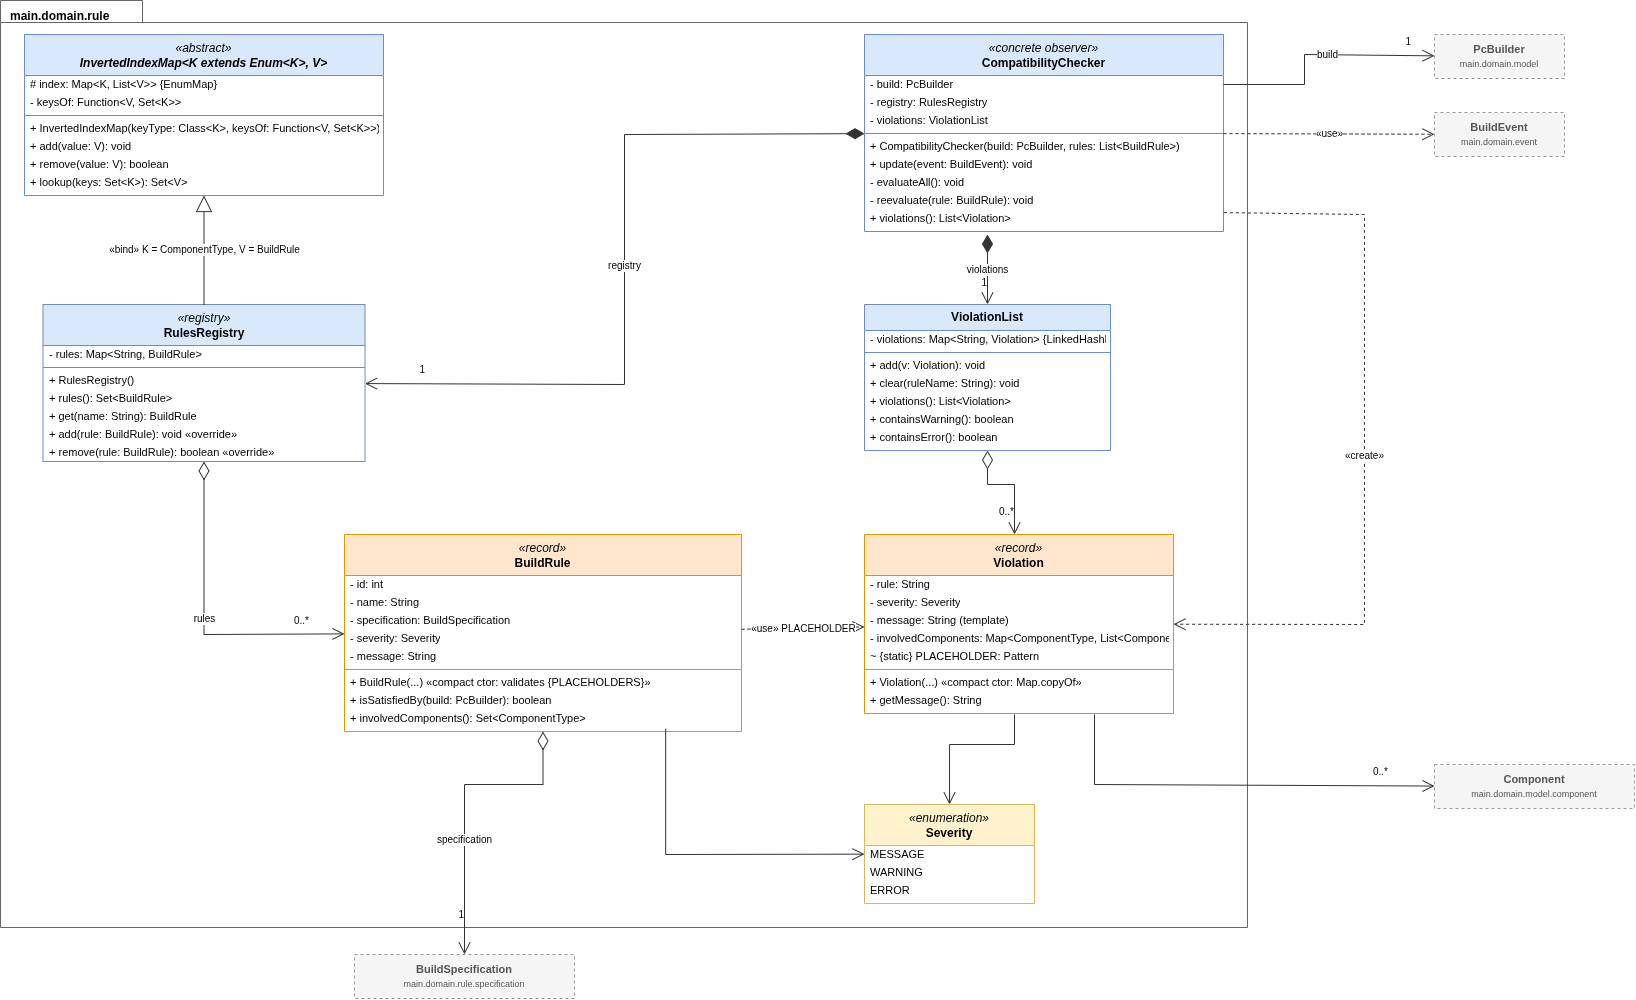
\includegraphics[width=1\linewidth]{diagrammi/model.rule.png}
    \caption{Enter Caption}
    \label{fig:placeholder}
\end{figure}


Il vero cuore di questa applicazione è il sistema di controllo per verificare le compatibilità tra i vari componenti. Ogni componente ha delle specifiche relative alle proprie dimensioni o tecnologie utilizzate (ad esempio le grandezze dei case e quindi cosa può effettivamente contenere o se il socket della cpu corrisponde con quello della scheda madre). Bisogna anche tenere conto se il numero di componenti inseriti è corretto o se manca un componente essenziale per poter utilizzare il pc.

\begin{lstlisting}[style=intellijlight, caption={A simple Java class}, label={lst:hello}]
//CompatibilityChecker.java
package main.domain.rule;

import java.util.*;

public class CompatibilityChecker implements Observer<BuildEvent> {
    private final PcBuilder build;
    private final RulesRegistry registry = new RulesRegistry();
    private final ViolationList violations = new ViolationList();

    public CompatibilityChecker(PcBuilder build, List<BuildRule> rules) {
        this.build = build;
        build.attach(this);
        // This lambda is the equivalent of r -> registry.add(r), it was suggested by the IDE
        rules.forEach(registry::add);
        evaluateAll();
    }

    @Override
    public void update(BuildEvent event) {
        if (event.type() == BuildEventType.RESTORED)
            evaluateAll();
        else {
            for (BuildRule rule : registry.lookup(Set.of(event.componentType()))) {
                reevaluate(rule);
            }
        }
    }

    private void evaluateAll() {
        for (BuildRule rule : registry.rules())
            reevaluate(rule);
    }

    private void reevaluate(BuildRule rule) {
        if (!rule.isSatisfiedBy(build)) {
            Map<ComponentType, List<Component>> involved = new LinkedHashMap<>();
            for (ComponentType type : rule.involvedComponents()) {
                involved.put(type, List.copyOf(build.getComponents(type)));
            }
            violations.add(new Violation(rule.name(), rule.severity(), rule.message(), involved));
        } else
            violations.clear(rule.name());
    }

    public List<Violation> violations() {
        return violations.violations();
    }
}

\end{lstlisting}

Il motore principale con il quale vengono create le regole di compatibiltà si basa sul design pattern \textit{Specification}: questo permette di definire business rules, con esito di validazione booleano, che possono essere combinate tra loro tramite operatori logici.

\subsection{Application}

\begin{figure}[H]
    \centering
    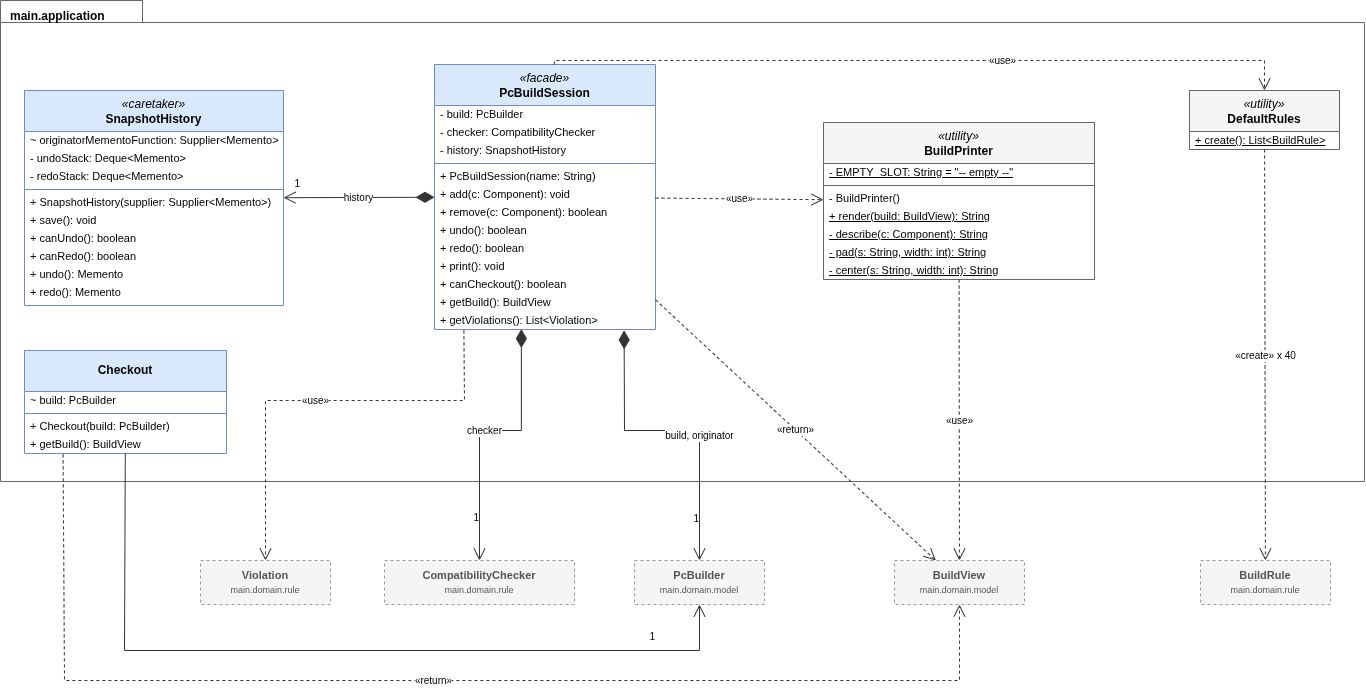
\includegraphics[width=1\linewidth]{diagrammi/application.png}
    \caption{Enter Caption}
    \label{fig:placeholder}
\end{figure}
Il pacchetto \texttt{application} contiene 

\subsection{ORM}
TODO

%\subsection{BusinessLogic}
%\subsubsection{LoginClieneteController e roba simile}

%\subsection{ORM (Object Relational Mapping}
%\subsubsection{ConnectionManager?? e roba simile}

%\subsection{Database}
%\subsection{Interfaccia}

\section{Design Pattern e Strutture Dati}

\subsection{Specification}
Specification è un design pattern definito da Eric Ewans in Domain Driven Design (da aggiungere ref).
\begin{itemize}
    \item \textbf{Problema}: "You need to check that only suitable objects are used for a certain role", si parla quindi di responsabilità di validazione.
    \item \textbf{Soluzione}: "Create a specification that is able to tell if a candidate  object matches some criteria. The specification has a method isSatisfiedBy(anObject): Boolean that returns "true" if all criteria are met by anObject".
\end{itemize}
Tra le varie implementazioni proposte, quella scelta è Composite Specification, che permette la massima flessibiltà e la possibilità di combinare le specifiche.

La struttura composita permette quindi di poter usare le operazioni di congiunzione logiche and e or) che compongono la specifica ad albero, con l'implementazione della versione composite di Specification si crea infatti un \textit{interpreter} per la lingua della specifiche. 
\begin{figure}[H]
    \centering
    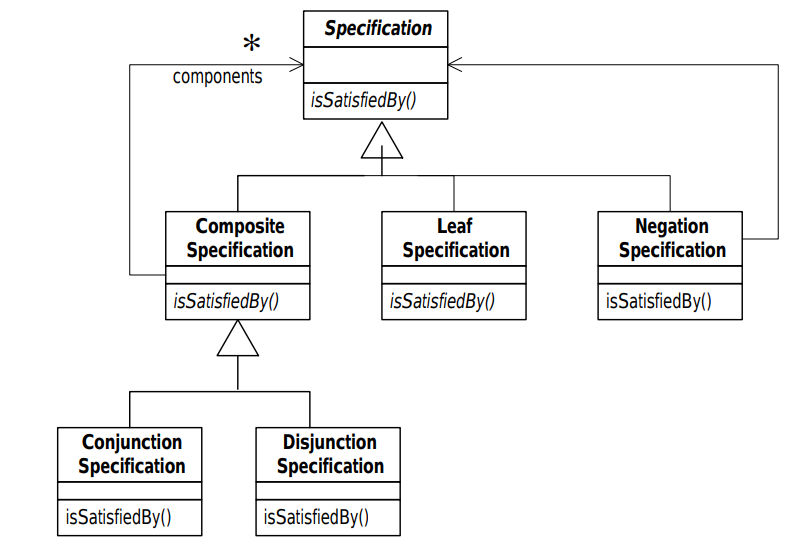
\includegraphics[width=0.5\linewidth]{diagrammi/specification.png}
    \caption{Enter Caption}
    \label{fig:placeholder}
\end{figure}

Grazie quindi alla caratteristica principale di un composite, ovvero quella di avere un interfaccia comune sia per i padri sia per le foglie nell'albero (in questo caso l'interfaccia è Specification), basta verificare la specifica risultante.

\begin{equation*}
\begin{aligned}
    \text{Esempio:} \quad & \text{SpecificationA} \land (\lnot\text{SpecificationB} \lor \text{SpecificationC}) \\
    \iff \quad & \texttt{SpecificationTot = SpecificationA.and(} \\
               & \quad \texttt{SpecificationB.not().or(SpecificationC))}
\end{aligned}
\end{equation*}

L'intera specifica potrà poi essere verificaza attravaerso 
\begin{equation*}
\begin{aligned}
    \texttt{SpecificationTot.isSatisfiedBy(Object)}
\end{aligned}
\end{equation*}

Specification permette quindi ti poter definire degli oggetti per validare la build in base alle specifiche, per poter sfruttarla al massimo però occorre ampliare la sua flessibilità:
\begin{enumerate}
    \item Nella sua definizione "standard", \texttt{isSatisfiedBy()} restituisce solo un booleano, quando nel caso dell'applicazione servono informazioni aggiuntive. Quindi le specifiche sono utilizzate per creare le \texttt{BuildRule}, che contengono quest'ultime, un nome, la gravità delle violazioni, i componenti coinvolti e degli eventuali messaggi da dare all'utente.\\
    Se queste regole sono violate, allora viene create una \texttt{Violation}, che contiene le informazioni sulla regola violata e la sua presenza (in caso di gravità \texttt{Severity.ERROR}) previene il checkout.

    \item Siccome le \textbf{BuildRule} hanno bisogno dei componenti che sono coinvolti nella loro specifica, ma l'atto di dover scrivere manualmente la lista \texttt{InvolvedComponents} esplicitamente riguardante più componenti è prono a errori. Entra quindi in gioco \texttt{BuildSpecification}, che aggiunge il metodo \texttt{dependsOn()} che grazie al meccanismo di \texttt{combine} è in grado di raccogliere tutte le dipendenze di componenti nell'albero composito della specifica.
    
\end{enumerate}

\begin{figure}[H]
    \centering
    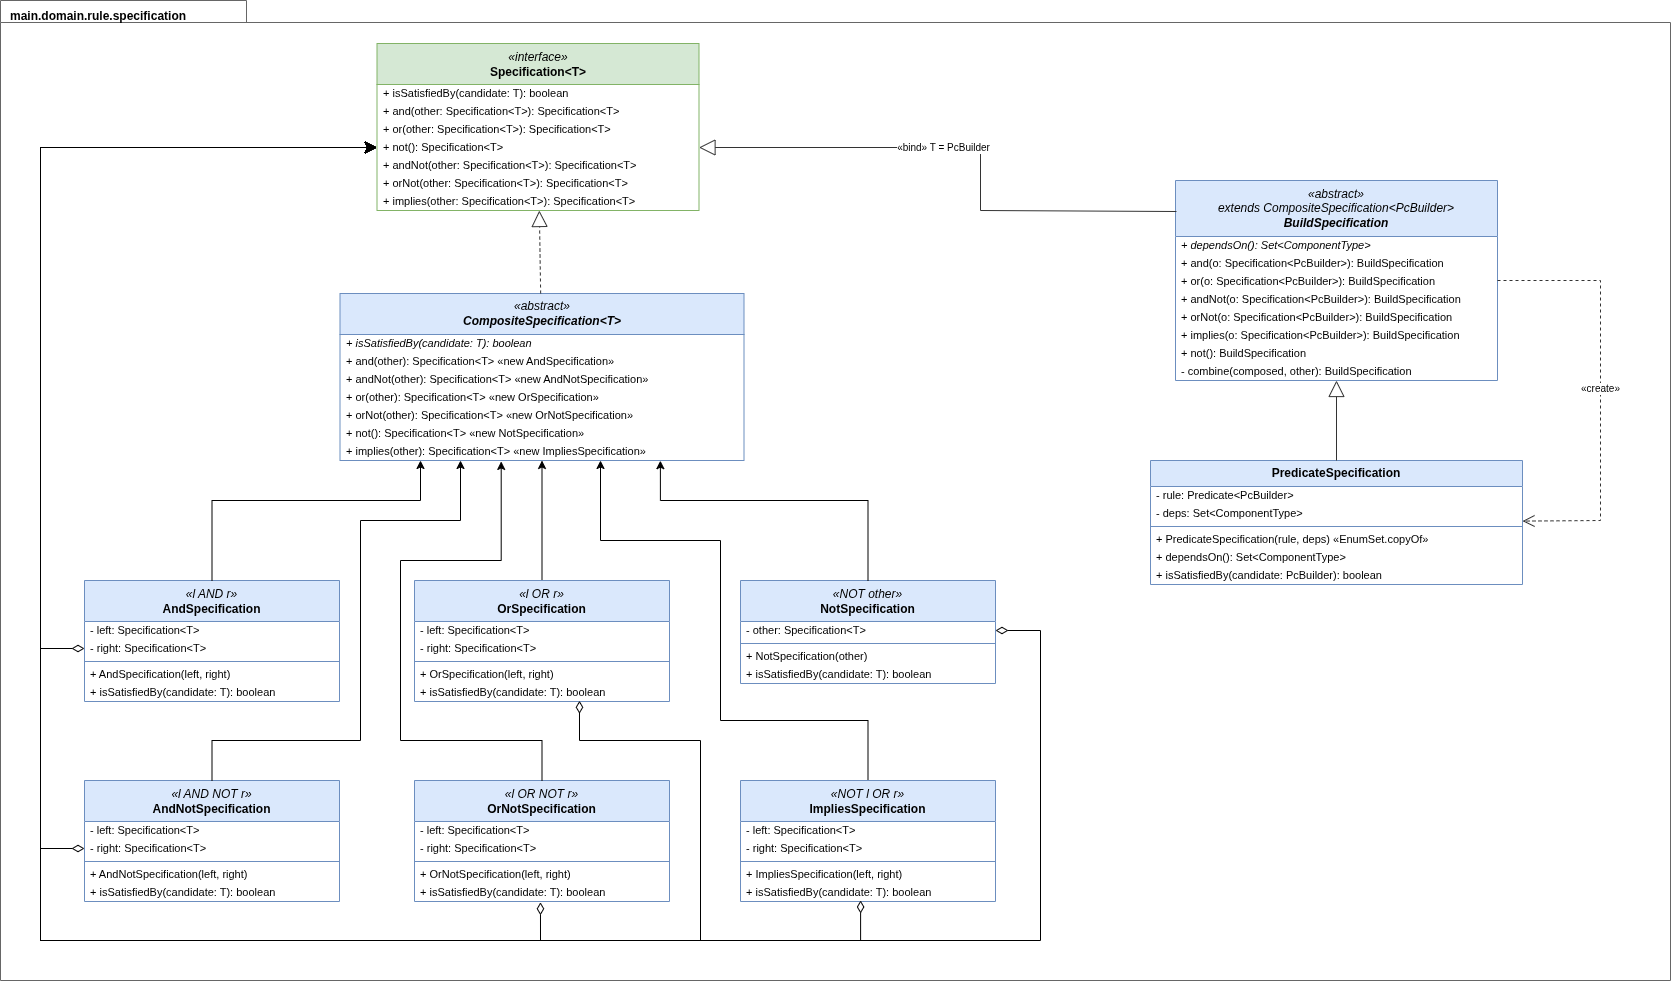
\includegraphics[width=1\linewidth]{diagrammi/pattern.specification.png}
    \caption{Enter Caption}
    \label{fig:placeholder}
\end{figure}

\begin{lstlisting}[style=intellijlight, caption={A simple Java class}, label={lst:hello}]
//Specification.java
package main.pattern.specification;

public interface Specification<T> {
    boolean isSatisfiedBy(T candidate);

    Specification<T> and(Specification<T> other);
    Specification<T> or(Specification<T> other);
    Specification<T> not();
    Specification<T> andNot(Specification<T> other);
    Specification<T> orNot(Specification<T> other);

    Specification<T> implies(Specification<T> other);

}

\end{lstlisting}

\begin{lstlisting}[style=intellijlight, caption={A simple Java class}, label={lst:hello}]
//CompositeSpecification.java
package main.pattern.specification;

public abstract class CompositeSpecification <T> implements Specification<T>{
    @Override public abstract boolean isSatisfiedBy(T candidate);
    @Override public Specification<T> and(Specification<T> other)    { return new AndSpecification<>(this, other); }
    @Override public Specification<T> andNot(Specification<T> other) { return new AndNotSpecification<>(this, other); }
    @Override public Specification<T> or(Specification<T> other)     { return new OrSpecification<>(this, other); }
    @Override public Specification<T> orNot(Specification<T> other)  { return new OrNotSpecification<>(this, other); }
    @Override public Specification<T> not()                          { return new NotSpecification<>(this); }
    @Override public Specification<T> implies(Specification<T> other) { return new ImpliesSpecification<>(this, other); }
}

\end{lstlisting}

\begin{lstlisting}[style=intellijlight, caption={A simple Java class}, label={lst:hello}]
//BuildSpecification.java
package main.domain.rule.specification;

public abstract class BuildSpecification extends CompositeSpecification<PcBuilder> {

    public abstract Set<ComponentType> dependsOn();

    @Override public BuildSpecification and(Specification<PcBuilder> o)     { return combine(super.and(o), o); }
    @Override public BuildSpecification or(Specification<PcBuilder> o)      { return combine(super.or(o), o); }
    @Override public BuildSpecification andNot(Specification<PcBuilder> o)  { return combine(super.andNot(o), o); }
    @Override public BuildSpecification orNot(Specification<PcBuilder> o)   { return combine(super.orNot(o), o); }
    @Override public BuildSpecification implies(Specification<PcBuilder> o) { return combine(super.implies(o), o); }
    @Override public BuildSpecification not() {
        return new PredicateSpecification(super.not()::isSatisfiedBy, dependsOn());
    }

    private BuildSpecification combine(Specification<PcBuilder> composed, Specification<PcBuilder> other) {
        if (!(other instanceof BuildSpecification b))
            throw new IllegalArgumentException(
                    "Cannot combine with a spec that does not declare its dependencies: " + other);
        Set<ComponentType> union = EnumSet.noneOf(ComponentType.class);
        union.addAll(dependsOn());
        union.addAll(b.dependsOn());
        return new PredicateSpecification(composed::isSatisfiedBy, union);
    }
}

\end{lstlisting}

\begin{lstlisting}[style=intellijlight, caption={A simple Java class}, label={lst:hello}]
//BuildRule.java
package main.domain.rule;

public record BuildRule (
                            int id,
                            String name,
                            BuildSpecification specification,
                            Severity severity,
                            String message
    ) {


    public BuildRule {
        Matcher m = Violation.PLACEHOLDER.matcher(message);
        while (m.find()) {
            ComponentType type;
            try {
                type = ComponentType.valueOf(m.group(1));
            } catch (IllegalArgumentException e) {
                throw new IllegalArgumentException("Rule " + name + ": unknown placeholder {" + m.group(1) + "}", e);
            }
            if (!specification.dependsOn().contains(type))
                throw new IllegalArgumentException("Rule " + name + ": placeholder {" + type + "} is not a component the rule depends on");
        }
    }

    public boolean isSatisfiedBy(PcBuilder build) {
        return specification().isSatisfiedBy(build);
    }

    public Set<ComponentType> involvedComponents() {
        return specification.dependsOn();
    }
}

\end{lstlisting}

\subsubsection{Creazione}
Una volta definiti tutti gli aspetti di Specification, bisogna definire le classi che vanno a definire effettivamente i requisiti in \texttt{isSatisfiedBy()}. Per evitare però di dover creare troppi file e rendere il progetto molto grande, le specifiche sono definite attraverso due classi "base":
\begin{enumerate}
    \item \textbf{ComponentCountSpecification}: ha come parametri il tipo di componente, il minimo e il massimo, \texttt{isSatisfiedBy(PcBuilder build)} quindi confronta la quantità di componenti inseriti nella lista di \texttt{type} con quelli forniti. \textit{Questo permette di avere una sola classe per tutte le specifiche che operano su una quantità di una categoria di componente}.
    \begin{lstlisting}[style=intellijlight, caption={A simple Java class}, label={lst:hello}]
package main.domain.rule.specification;

public final class ComponentCountSpecification extends BuildSpecification {
    private final ComponentType type;
    private final int min, max;

    public ComponentCountSpecification(ComponentType type, int min, int max) {
        this.type = type;
        this.min = min;
        this.max = max;
    }

    @Override
    public boolean isSatisfiedBy(PcBuilder build) {
        int n = build.getComponentNumber(type);
        return n >= min && n <= max;
    }

    @Override public Set<ComponentType> dependsOn() { return EnumSet.of(type); }
}


    \end{lstlisting}
    \item \textbf{PredicateSpecification}: ha come parametri un \textit{Predicate} e i componenti dai quali dipende. Predicate è un'interfaccia funzionale di java che permette di definire un predicato e poterlo verificare con \texttt{.test()}. \textit{Questo permette di avere una sola classe per tutte le specifiche che necessitano di un predicato per essere verificate}.
    \begin{lstlisting}[style=intellijlight, caption={A simple Java class}, label={lst:hello}]
package main.domain.rule.specification;

public class PredicateSpecification extends BuildSpecification {

    private final Predicate<PcBuilder> rule;
    private final Set<ComponentType> deps;

    public PredicateSpecification(Predicate<PcBuilder> rule, Set<ComponentType> deps) {
        this.rule = rule;
        this.deps = deps.isEmpty() ? Set.of() : EnumSet.copyOf(deps);
    }

    @Override
    public Set<ComponentType> dependsOn() {
        return deps;
    }

    @Override
    public boolean isSatisfiedBy(PcBuilder candidate) {
        return rule.test(candidate);
    }
}

    \end{lstlisting}
\end{enumerate}

Come si può notare queste due classi di specifiche sono le \textbf{uniche non astratte}, quindi si possono creare istanze di specifiche \textbf{solo} secondo queste due tipologie e caratteristiche.

L'unico passaggio rimasto è quello di scrivere tutti gli oggetti necessari, che vengono definiti dentro \texttt{Specs}:
\begin{enumerate}
    \item \texttt{ComponentCountSpecification} viene utilizzato per creare i metodi<z\textit{factory} \texttt{atMost}, \texttt{atLeast}, e \texttt{excacltyOne} (oltre a \texttt{multipleExcactlyOne} che verrà spiegato nella sezione successiva). Questi metodi prendeno come parametro il tipo di componente ed un valore numerico
    \begin{lstlisting}[style=intellijlight, caption={A simple Java class}, label={lst:hello}]
    //Specs.java
    public static BuildSpecification atMost(ComponentType t, int n)  { return new ComponentCountSpecification(t, 0, n); }
    public static BuildSpecification atLeast(ComponentType t, int n) { return new ComponentCountSpecification(t, n, Integer.MAX_VALUE); }
    public static BuildSpecification exactly(ComponentType t, int n) { return new ComponentCountSpecification(t, n, n); }

    public static BuildSpecification mutipleExcatclyOne(ComponentType... t) {
        BuildSpecification res = new ComponentCountSpecification(t[0], 1, 1);
        for (int i = 1; i < t.length; i++)
            res = res.and(new ComponentCountSpecification(t[i], 1, 1));
        
        return res;
    }
    \end{lstlisting}

    \item Le specification con predicati vengono create come oggetti di classe \texttt{PredicateSpecification}, dove il predicato di \texttt{isSatisfiedBy()} viene dichiarato direttamente nel costruttore, utilizzando le funzioni lambda (che verranno poi eseguite quandi si andrà a fare \texttt{Predicate.test()}.
    \begin{lstlisting}[style=intellijlight, caption={A simple Java class}, label={lst:hello}]
    //Specs.java
    public static BuildSpecification socketMatchSpecification = new PredicateSpecification(
            b -> b.getSingleComponent(ComponentType.CPU, Cpu.class).socket().equals(b.getSingleComponent(ComponentType.MOTHERBOARD, Motherboard.class).socket()),
            Set.of(ComponentType.CPU, ComponentType.MOTHERBOARD)
    );

    public static BuildSpecification gpuLengthFitsCaseSpecification = new PredicateSpecification(
            b -> b.getComponents(ComponentType.GPU, Gpu.class).stream().allMatch(g -> g.lenghtMm() <= b.getSingleComponent(ComponentType.CASE, Case.class).maxGpuLengthMm()),
            Set.of(ComponentType.GPU, ComponentType.CASE)
    );

    ...
    
    \end{lstlisting}
\end{enumerate}

\subsubsection{Logica}
Le regole sono tutte instanziate dentro il regitrso \texttt{RulesRegistry}, la quale struttra e funzionamento verrà spiegato nella sezione riguardanti le strutture dati. \\
Le regole vengono verificate da \texttt{CompatibilityChecker} con i metodi \texttt{evaluateAll()} e \texttt{reevaluate()}.

Se ogni singola regola venisse valutata senza nessun meccanismo di guardia si avrebbero che messaggi di violazioni per stati nel quale la build non è, per esempio: non si può avere un messaggio "Il socket della CPU non corrisponde con quello della MOBO" se una delle due è mancante. Inoltre, sia per il meccanismo di placehoder dei messaggi e di alcuni metodi usati come \texttt{build.getSingleComponent} (che può lanciare un'eccezione) producono degli errori se eseguiti senza un controllo.

Per esempio, se si volesse controllare se il socket corrisponde tra CPU e scheda madre oppure quando una o entrambe le due sono mancanti, si sta cercando di effettuare delle operazioni con degli oggetti in uno stato non corretto (in quando non si sono verificate le precondizioni): si ha infatti \texttt{IllegalStateException}.\\
Stessa cosa accade anche nel secondo esempio, sempre per la mancanza di una cpu nella build.
\begin{table}
    \centering
    \footnotesize
    \begin{tabularx}{\textwidth}{|X|X|}
    \hline
    \ttfamily
    new BuildRule(\newline
    \hspace*{2em}14,\newline
    \hspace*{2em}"SOCKET-MISMATCH",\newline
    \hspace*{2em}Specs.socketMatchSpecification,\newline
    \hspace*{2em}Severity.ERROR,\newline
    \hspace*{2em}"CPU \{CPU\} and Motherboard \{MOTHERBOARD\} socket must match"\newline
    ), & 
    \ttfamily\color{red!80!black}
    Exception in thread "main" java.lang.IllegalStateException: No component found for type: CPU \\
    \hline
    \ttfamily
    new BuildRule(\newline
    \hspace*{2em}13,\newline
    \hspace*{2em}"MISSING-COOLER",\newline
    \hspace*{2em}Specs.cpuHasBundledCoolerSpecification
    \hspace*{2em}.or(Specs.atLeast(ComponentType.COOLING, 1),\newline
    \hspace*{2em}Severity.ERROR,\newline
    \hspace*{2em}"CPU \{CPU\} ships without a cooler and none was selected"\newline
    ), & 
    \ttfamily\color{red!80!black}
    Exception in thread "main" java.lang.IllegalStateException: No component found for type: CPU \\
    \hline
    \end{tabularx}
    \caption{Esempi di regole ed eccezioni corrispondenti.}
    \label{tab:buildrule_exception}
\end{table}

                


Come meccanismo di guardia per evitare le problematiche menzionate, è stato aggiunto \texttt{implies()} agli operatori logici di Specification:
\begin{equation*}
    A \rightarrow B \quad\iff\quad  \lnot A \lor B
\end{equation*}

L'aspetto fondamentale da considerare quando si parla di operatori logici in linguaggi di programmazione è quello dello \textit{short-circuit}, ovvero corto circuito:

\begin{quote}
    La valutazione a corto circuito, valutazione minima o valutazione di McCarthy è un meccanismo relativo agli operatori booleani binari per cui il secondo operando viene valutato unicamente se il valore del primo operando non è sufficiente da solo a determinare il risultato dell'espressione: quando il primo argomento dell'operatore logico AND è falso, il valore dell'intera espressione dovrà essere necessariamente falso; e quando il primo argomento dell'operatore logico OR è vero, il valore dell'intera espressione dovrà essere necessariamente vero. \href{https://it.wikipedia.org/wiki/Valutazione_a_corto_circuito}{wikipedia da citare}
\end{quote}

Appurato questo aspetto fondamentale, si può adesso entrare nei dettagli di come l'implicazione fa da guardia. Se si prendono due variabili booleane \(A\) e \(B\) e si valuta \(A\rightarrow B\):
\begin{itemize}
    \item Se \(A\) è vero, allora l'espressione diventa \[\lnot \mathrm{True}\lor B\quad \iff \quad B \] e dipende \textit{unicamente} dal valore di \(B\).
    \item Se \(A\) è falso, allore l'espressione diventa \[\lnot \mathrm{False}\lor B \quad \iff \quad \mathrm{True} \lor B\]ma per il cortocircuito \(B\) viene ignorata e di conseguenza non viene neanche valutata, dando direttamente come risultato \textrm{True}.
\end{itemize}

\subsubsection{Composizione con Guardie}
Una volta definita la logica dietro il meccanismo dell'implicazione utilizzando il cortocircuito, si passa all'applicazione di questa nel codice, per creare delle specifiche con guardia.

Data la specifica di guardia \texttt{GuardSpecification},  la  specifica che si vuole valutare \texttt{ActualSpecification} e la loro composizione \texttt{ResultSpecification = GuardSpecification.implies(ActualSpecification)}, nel codice si hanno le seguenti conseguenze sul risultato di \texttt{ResultSpecification.isSatisfiedBy(Object)}:

\begin{itemize}
    \item Se \texttt{GuardSpecification.isSatisfiedBy(Object) == True}, allora \newline\texttt{ResultSpecification.isSatisfiedBy(Object)} dipende \textit{unicamente} dall'esito di \texttt{ActualSpecification.isSatisfiedBy(Object)}
    \item Se \texttt{GuardSpecification.isSatisfiedBy(Object) == False}, allora per il cortocircuito logico \texttt{ResultSpecification.isSatisfiedBy(Object)} ha come esito \texttt{True}, ma sopratutto \textbf{non viene invocato} il metodo \newline\texttt{ActualSpecification.isSatisfiedBy(Object)}.
\end{itemize}

Quindi in conclusione, quando vengono valutate delle regole che presentano una guardia, se l'esito è negativo allora si trovano in uno stato nel quale questa è valutabile, e può generare conseguentemente le relative \texttt{Violation}. Nel caso sia vera invece, o la specifica è in uno stato valutabile e risulta rispettata, oppure è in uno stato non valutabile, ma dando come risultato \texttt{True} questa valutazione è \textbf{trasparente} e non genera nessuna \texttt{Violation} (e si prevengono tutte le problematiche iniziali). 

Riprendendo l'esempio precedente (quello della tabella, da aggiungere refernce), si riscrivono le regole nel seguente modo:
\begin{lstlisting}[style=intellijlight, caption={A simple Java class}, label={lst:hello}]
new BuildRule(
    14,
    "SOCKET-MISMATCH",
    Specs.mutipleExcatclyOne(ComponentType.CPU, ComponentType.MOTHERBOARD).implies(Specs.socketMatchSpecification),
    Severity.ERROR,
    "CPU {CPU} and Motherboard {MOTHERBOARD} socket must match"
),
new BuildRule(
    12,
    "MISSING-COOLER",
    Specs.excatcly(ComponentType.CPU, 1).implies(Specs.cpuHasBundledCoolerSpecification.or(Specs.atLeast(ComponentType.COOLING, 1))),
    Severity.WARNING,
    CPU {CPU} ships without a cooler and none was selected"
),
\end{lstlisting}

\subsection{Observer}
L'implementazione di \texttt{Observer} è quella standard di GoF, con la sola differenza che le interfaccie sono dichiarate in modo generico e viene utilizzato un oggetto apposito per la notifica (\texttt{Event}).
\begin{figure}[H]
    \centering
    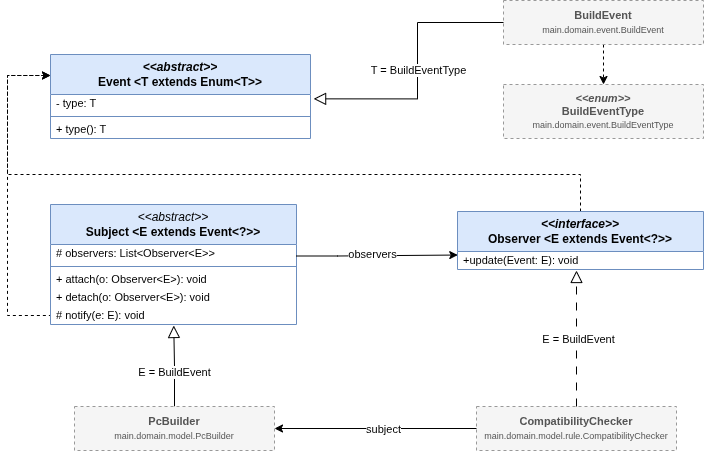
\includegraphics[width=1\linewidth]{diagrammi/observer.png}
    \caption{Enter Caption}
    \label{fig:placeholder}
\end{figure}
Questa scelta di implementazione è simile a quella di \textit{EventListener} in java, dove invece di avere solamente un \textit{push} o un \textit{pull}, vengono effettuati entrambi: viene effettuato un push dell'oggetto \texttt{Event} in base al quale poi gli oggetti \texttt{Observer} possono attingere ai dati di \texttt{Subject}.

Quando \texttt{notify()} viene chiamato dentro \texttt{PcBuilder} (nei metodi \texttt{addComponent()}, \texttt{removeComponent()} e \texttt{RestoreMemento()}), viene effettuato un push di un \texttt{BuildEvent}, per esempio \texttt{notify(new BuildEvent(BuildEventType.ADDED, c));}

Dopodichè l'evento viene passato a \texttt{CompatibilityChecker} (ovvero l'Observer) che col metodo \texttt{update()} provvede ad elaborare l'evento

\begin{lstlisting}[style=intellijlight, caption={A simple Java class}, label={lst:hello}]
    @Override
    public void update(BuildEvent event) {
        if (event.type() == BuildEventType.RESTORED)
            evaluateAll();
        else {
            for (BuildRule rule : registry.lookup(Set.of(event.componentType()))) {
                reevaluate(rule);
            }
        }
    }
\end{lstlisting}

Siccome la lista delle BuildRule è molto grande, per evitare di dover ogni volta rielaborare ognuna di esse, si controlla se l'evento è di tipo \texttt{BuildEventType.ADDED o .REMOVED}. Se è questo il caso, si procede alla rivalutazione solo delle regole legate al componente che è stato aggiunto o rimosso, sfruttando la \texttt{InvertedIndexMap} di \texttt{BuildRegistry}:

\begin{verbatim}
PcBuildSession.add(c)
  -> PcBuilder.addComponent(c)
       components.get(c.type()).add(c);                    // 1. mutate state
       notify(new BuildEvent(ADDED, c));                   // 2. then notify
         -> CompatibilityChecker.update(event)
              registry.lookup(Set.of(event.componentType()))   // 3. dirty set
              -> reevaluate(rule) for each                     // 4. re-check
\end{verbatim}
Nel caso invece che l'evento sia quello di \texttt{RESTORED}, vengono rivalutate tutte le regole.

Insieme a Specification, Observer è un altro componente fondamentale dell'applicazione, questo duo è responsabile della maggior parte della logica.

\subsection{Memento}
Il design pattern Memento serve a salvare gli stati interni della build, che in questo caso sono utilizzati per implementare le azioni di \textit{undo/redo}(Ctrl+Z/Ctrl+Y). L'implementazione cerca di seguire il più possibile quella standard di GoF, ma siccome manca l'operatore \textit{friend} del C++ si ricorre ad un altro meccanismo per garantire che lo stato registrato da uno snapshot sia accessibile solo dall'Originator: \texttt{BuildSnapshot} implementa l'interfaccia \texttt{Memento} (anche se vuota) e aggiunge il metodo \texttt{getState()}. Così facendo \texttt{SnapshotHistory} opera su l'interfaccia \texttt{Memento} e non  conosce l'esistenza della classe privata interna \texttt{PcBuilder.BuildSnaphot}, ma quando l'oggetto \texttt{Memento} viene passato come argomento a \texttt{PcBuilder.restoreMemento(Memento)}, quest'utlimo può accedera allo stato nascosto tramite un cast a \texttt {BuildSnapshot}.
\begin{figure}[H]
    \centering
    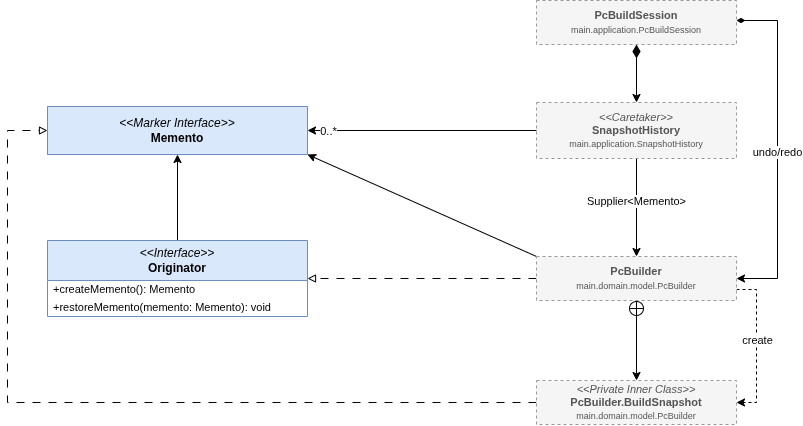
\includegraphics[width=1\linewidth]{diagrammi/memento.png}
    \caption{Enter Caption}
    \label{fig:placeholder}
\end{figure}Occore inoltre fare un confronto col design pattern \texttt{Command}...

\subsection{Facade}
Per quanto riguarda l'utilizzo da parte dell'utente finale, conviene semplificare tutti i meccanismi dell'applicazione in un'unica interfaccia unificata al sottosistema, che funge quindi da \texttt{Facade}. Questo fa si che l'utente non deva accedere ai singoli oggetti che compongono l'applicazione, ma si interfaccia a \texttt{PcBuildSession} che semplifica l'accesso a quest'ultimi, ma che comunque non lo priva se necessario.  

I vantaggi che si ottengono sono i seguenti:
\begin{itemize}
    \item Disaccoppiamento tra il client e il sistema, permettendo maggiore flessibilità.
    \item Permette di effettuare controlli aggiuntivi sulle azioni degli utenti e preserva le invarianti (come per esempio quella di eseguire \texttt{save()} ad ogni cambiamento).
    \item Restituisce solo una \texttt{BuildView} della build come risultato.
    \item Crea un livello di astrazione \textit{Application Layer}.
\end{itemize}
\begin{figure}[H]
    \centering
    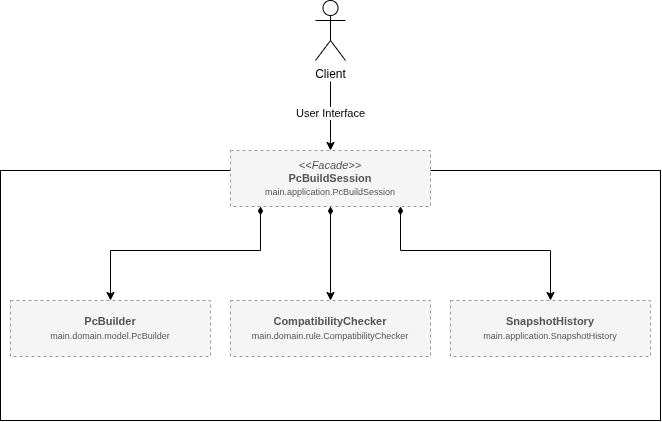
\includegraphics[width=1\linewidth]{diagrammi/facade.png}
    \caption{Enter Caption}
    \label{fig:placeholder}
\end{figure}

\subsection{Altri Design Pattern}
\begin{itemize}
    \item \textbf{Factory}
    \item \textbf{Proxy}
    \item \textbf{Interpreter}
\end{itemize}
\subsection{Strutture Dati Utilizzate}
La struttura dati principale, che rappresenta la build del pc, è una \texttt{EnumMap<>}, che ha come chiavi i tipi di componenti, e come valori le liste di quei componenti.
\begin{figure}[H]
    \centering
    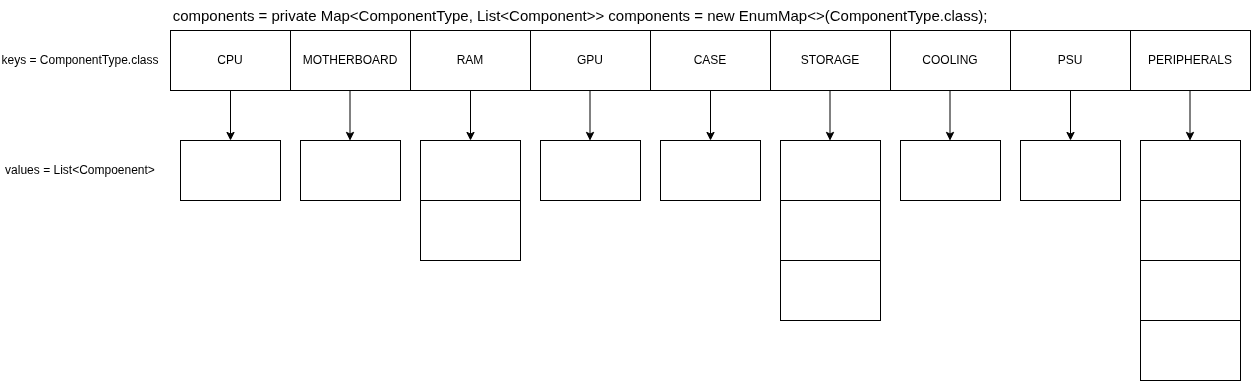
\includegraphics[width=1\linewidth]{diagrammi/components.png}
    \caption{Enter Caption}
    \label{fig:placeholder}
\end{figure}

Per quanto riguarda invece le strutture dati di supporto alle regole, si hanno due strutture dati.
La prima \texttt{LinkedHasehdMap<>}, indicizzata tramite il nome (univoco) della regole e contiene la regola stessa. Questa è la struttura "base" delle regole, e la mappa serve per potere accederci direttamente tramite il loro nome per le varie operazioni che si possono effettuare su di esse (aggiunta e rimozione).
\begin{figure}[H]
    \centering
    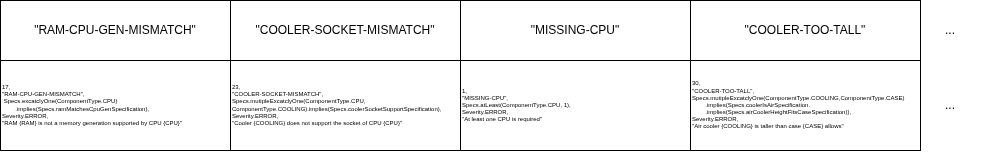
\includegraphics[width=1\linewidth]{diagrammi/rules.png}
    \caption{Enter Caption}
    \label{fig:placeholder}
\end{figure}
La seconda invece inverte la mappa, prendendo un altra chiave ovvero i componenti presenti in \texttt{BuildRule.involvedComponents}. La struttura è definita in \texttt{InvertedIndexMap}

\begin{lstlisting}[style=intellijlight, caption={A simple Java class}, label={lst:hello}]
//InvertedIndexMap.java
package main.domain.rule;


public abstract class InvertedIndexMap<K extends Enum<K>, V> {

    protected final Map<K, List<V>> index;
    private final Function<V, Set<K>> keysOf;

    public InvertedIndexMap(Class<K> keyType, Function<V, Set<K>> keysOf) {
        this.index = new EnumMap<>(keyType);
        this.keysOf = keysOf;
        for(K key : keyType.getEnumConstants()) {
            index.put(key, new ArrayList<>());
        }
    }

    public void add(V value) {
        Set<K> keys = keysOf.apply(value);
        for (K key : keys) 
            index.get(key).add(value);
    }

    public boolean remove(V value) {
        boolean removed = false;
        Set<K> keys = keysOf.apply(value);
        for (K key : keys) {
            // Keys are pre-initialized in the constructor and never removed, so the list is always present.
            removed |= index.get(key).remove(value);
        }
        return removed;
    }

    public Set<V> lookup(Set<K> keys) {
        // VERY Important that this is a set, we don't want repeting values coming from different keys
        Set<V> result = new LinkedHashSet<>();
        keys.forEach(k -> result.addAll(index.getOrDefault(k, List.of())));
        return result;
    }

}

\end{lstlisting}

\begin{figure}[H]
    \centering
    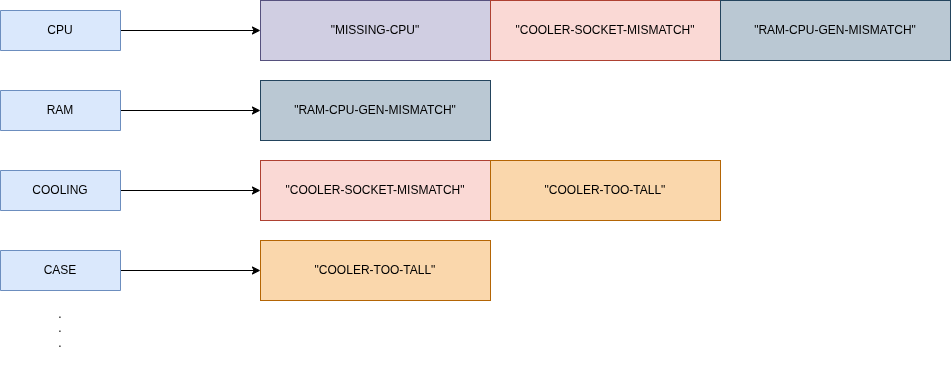
\includegraphics[width=1\linewidth]{diagrammi/invertedindex.png}
    \caption{Enter Caption}
    \label{fig:placeholder}
\end{figure}
Quindi la mappa si basa sempre su una \texttt{EnumMap<>} come \texttt{components}, ma i valori sono tutte le regole che tra i componenti coinvolti contengono anche quello dell'indice. Per questa definizione ci saranno quindi dei duplicati nei valori, ovvero le regole che dipendono da due o più componenti.

Quando si va ad aggiungere/rimuovere/rimpiazzare un componente, vengono prese in considerazioni \textbf{solo} le regole che comprendono quella tipologia di componente (...), in modo da non dover rivalutare tutta la lista di regole.
%\section{Testing}
%\subsection{Business Logic Test}
%\subsubsection{LoginControllerTest}

%\subsection{Domain Model Test}
%\subsection{ORM Test}

\end{document}